\section{The models}
\label{models}





\subsection{Quantum many-body systems}
\label{quamod}

As a paradigmatic quantum many-body system we consider the 1D quantum
Ising models, described by the Hamiltonian
\begin{eqnarray}
  H_{qI}(g,h) = - J \sum_{x=1}^{L} \sigma^{(1)}_{x\phantom{1}}
  \sigma^{(1)}_{x+1} - g \sum_{x=1}^L \sigma^{(3)}_x
  - h \sum_{x=1}^L \sigma^{(1)}_x\,,\quad
  \label{qisingmodel}
\end{eqnarray}
where $L$ is the system size, $\sigma^{(k)}_x$ are the Pauli matrices
on the $x^{\rm th}$ site ($k = 1,2,3$ labels the three spatial
directions). Periodic and antiperiodic boundary conditions
(respectively PBC and ABC) are set by requiring respectively
$\sigma^{(k)}_{L+1} = \sigma^{(k)}_1$ and $\sigma^{(k)}_{L+1} =
-\sigma^{(k)}_1$.

We recall that the quantum Ising model (\ref{qisingmodel}) develops a
quantum critical behavior at $g=g_c=J$ and $h=0$, belonging to the 2D
Ising universality class, see e.g. Ref.~\cite{Sachdev-book}. The model
is always gapped for $h\neq 0$.  The relevant parameters $r\equiv
g-g_c$ and $h$ are respectively associated with even and odd RG
perturbations at the Ising fixed point.  Their RG dimensions are
respectively $y_r=1/\nu=1$ and $y_h=15/8$. The dynamic exponent $z$,
controlling the vanishing of the gap at the transition point, is given
by $z=1$. Moreover, we recall that the RG dimension of the
order-parameter field, associated with the longitudinal operators
$\sigma_x^{(1)}$, is given by $y_l=d + z - y_h=1/8$, while that
associated with the transverse operator $\sigma_x^{(3)}$ is given by
$y_t = d + z - y_r = 1$.  In the following we assume ferromagnetic
nearest-neighbour interactions with $J=1$, thus $g_c=J=1$.


To achieve round-trip protocols between gapped phases, without
degeneration of the lowest quantum states, we consider Ising chains
with PBC at $g=g_c$ driven by a time-dependent longitudinal field
$h(t)$, that is,  comparing with Eq.~(\ref{hlamt}), we identify
\begin{eqnarray}
  H_c = H_{qI}(g_c,0)\,,\quad w(t) = h(t)\,, \quad H_p = - \sum_{x}
  \sigma^{(1)}_x\,.
\label{isichoice}
\end{eqnarray}

The quantum Ising Hamiltonian $H_{qI}(g,0)$ for vanishing longitudinal
field $h$ can be mapped into a quadratic model of spinless fermions
through a Jordan-Wigner transformation~\cite{LSM-61, Katsura-62},
obtaining the so-called quantum Kitaev wire:~\cite{Kitaev-01}
\begin{equation}
  H_{K}(\mu) = - \sum_{x} \big( c_x^\dagger c_{x+1} + c_x^\dagger
  c_{x+1}^\dagger + {\rm h.c.}  \big) - \mu \sum_{x} n_x \,,
  \label{kitaev2}
\end{equation}
where $c_x^{(\dagger)}$ is the fermionic annihilation (creation)
operator on site $x$ of the chain, $n_x\equiv c_x^\dagger c_x$ is the
corresponding number operator, and $\mu=-2g$.  Analogously to the
Ising spin representation, PBC and ABC are set by requiring
respectively $c_{L+1} = c_1$ and $c_{L+1} = -c_1$.  The Kitaev model
undergoes a continuous quantum transition at $\mu_c = -2g_c = -2$.  Of
course, it belongs to the 2D Ising universality class as well, so that
$y_\mu= y_r = 1/\nu=1$ (there is no an analogue of the longitudinal
field $h$ of the spin formulation (\ref{qisingmodel}) within the above
fermionic representation).  At the Ising transition the fermionic
operators $c_x$ and the particle density operator $n_x$ acquire the RG
dimensions $y_c=1/2$ and $y_n=1$, respectively.


Although the bulk behaviors of the Ising and Kitaev models in the
infinite-volume limit (and thus their phase diagram) are analogous,
some features of finite-size systems may significantly differ.  As a
matter of fact, the nonlocal Jordan-Wigner transformation of the Ising
chain with PBC or ABC does not simply map into the fermionic
model~\eqref{kitaev2} with PBC or ABC.  Indeed further considerations
apply~\cite{Katsura-62, Pfeuty-70}, leading to a less straightforward
correspondence, which also depends on the parity of the
particle-number eigenvalue. In particular, we note that the Kitaev
quantum wire with ABC turns out to be gapped in both phases separated
by the quantum transition at $\mu_c=-2$. Indeed, it does not exhibit
the lowest-state degeneracy of the ordered phase of the quantum Ising
chain (namely, the exponential suppression of the gap with increasing
$L$).  The reason for such substantial difference resides in the fact
that the Hilbert space of the former is restricted with respect to
that of the latter, so that it is not possible to restore the
competition between the two vacua belonging to the
symmetric/antisymmetric sectors of the Ising model~\cite{Katsura-62,
  Kitaev-01, CPV-14, RV-21}.  Therefore, a continuous quantum
transition between gapped phases is also realized within the Kitaev
wire with ABC, by choosing
\begin{eqnarray}
  H_c = H_K(\mu_c)\,,\quad w(t) = \mu(t)-\mu_c\,,
  \quad H_p = - \sum_{x} n_x\,.\;\;
\label{kitchoice}
\end{eqnarray}


\subsection{Classical Ising model}
\label{classmod}

As a classical paradigmatic model undergoing a finite-temperature
continuous transition, we consider the 2D Ising model,
defined on a square lattice by the partition function
\begin{eqnarray}
  &&Z = \sum_{\{s_{\bm x}\}} e^{-\beta H_{cI}}\,,\qquad
  \beta=1/T\,, \label{partfunc}\\
  &&H_{cI}(J,h) = - J \sum_{\langle
    {\bm x} {\bm y} \rangle} s_{\bm x} s_{\bm y} - h
  \sum_{\bm x}
  s_{\bm x}\,,
\label{classisi}  
\end{eqnarray}
where ${\bm x}$ are the sites of the lattice, ${\langle {\bm x} {\bm
    y} \rangle}$ indicates the nearest-neighbour sites of the lattice,
$s_{\bm x}=\pm 1$ are classical spin variables, and $h$ is an external
homogenous magnetic field (we use the same symbol of the external
longitudinal field of the quantum ising model (\ref{qisingmodel}), but
this should not lead to confusion). We consider systems with PBC.  We
again set $J=1$.  The square-lattice Ising model (\ref{classisi})
undergoes a thermal continuous transition at $h=0$ and
$T_c=2/\ln(\sqrt{2}+1)$~\cite{Onsager-44}.  The critical behavior
belongs to the same universality class of the 1D quantum Ising
model. Therefore, it is characterized by the critical exponents
$\nu=1$ and $\eta=1/4$, and correspondingly the RG dimension
associated with the temperature relevant parameter is given by
$y_t=1/\nu=1$, and that associated with the odd external field $h$ is
$y_h = 2-\eta/2=15/8$, see e.g. Ref.~\cite{PV-02}.

Since we are going to discuss dynamic behaviors, we must also define
the type of dynamics driving the time evolution of the system.  We
consider a purely relaxational dynamics (also known as model A of
critical dynamics~\cite{HH-77,Ma-book}), which can be realized by stocastic
Langevin equations, or just Metropolis updatings in Monte Carlo
simulations~\cite{Metropolis:1953am}.  The corresponding dynamic
exponent $z$ has been accurately estimated by numerical studies,
obtaining $z\approx 2.167$ with an apparent relative precision that is
better than one per mille. Indeed, some of the most recent estimates
of the dynamic exponent $z$ for purely relaxational dynamics are
$z=2.1667(5)$ from \cite{NB-00}, $z=2.168(5)$ from \cite{WH-97},
$z=2.1665(12)$ from \cite{NB-96}, $z=2.172(6)$ from \cite{G-95},
$z=2.170(6)$ from Ref.~\cite{CV-11}, which have been obtained by
numerical analyses based on Monte Carlo simulations in equilibrium
conditions. In the following we use the estimate $z=2.167(1)$.

One may consider time-dependent KZ protocols also in this classical
context, supplementing the partition function (\ref{partfunc})
defining the classical Ising model with the purely relaxational
dynamics.  Analogously to the quantum case, cf. Eq.~(\ref{isichoice}),
we consider 2D Ising models with PBC at $T_c$ driven by a
time-dependent magnetic field $h(t)$. Therefore, we identify
\begin{eqnarray}
  & H_c = H_{cI}(1,0)\,,\qquad &\beta=\beta_c = {\ln(\sqrt{2}+1)\over
    2} \,, \label{clisichoice}\\ & w(t) = h(t)\,, \qquad &H_p
  = - \sum_{\bm x} s_{\bm x}\,.\nonumber
\end{eqnarray}



\section{One-way and round-trip KZ protocols across transition points}
\label{protocols}


In the following we assume the general Hamiltonian (\ref{hlamt}),
which represents the three models presented in Sec.~\ref{models} with
the identifications in Eqs.~(\ref{isichoice}), (\ref{kitchoice}), and
(\ref{clisichoice}).


\subsection{One-way KZ protocols}
\label{oneway}


KZ-like protocols have been largely employed to investigate the
dynamics of critical systems, at quantum transitions when the
many-body system is subject to unitary time evolutions, and at
classical thermal transitions considering, for example, a purely
relaxational dynamics which can be implemented by standard Langevin
equations~\cite{HH-77}.

\subsubsection{Quantum KZ protocols}
\label{quoneway}

In the case of quantum many-body systems, quasi-adiabatic passages
through the continuous quantum transition are obtained by slowly
varying $w$ across $w_c = 0$, following, e.g., the standard KZ
procedure:

(i) One starts from the ground state of the many-body system at
  $w_i < 0$, that is $|\Psi(t=0)\rangle \equiv |\Psi_0(w_i)\rangle$.
  
(ii) Then the out-of-equilibrium unitary dynamics, ruled by the
Schr\"odinger equation
  \begin{equation}
    {{\rm d} \, |\Psi(t)\rangle \over {\rm d} t} =
    - i \, \hat H[w(t)] \, |\Psi(t)\rangle \,,
    \label{unitdyn}
  \end{equation}
  arises from a linear time dependence of the Hamiltonian parameter
  $w(t)$, such as
  \begin{equation}
    w(t) = t/t_s \,,
    \label{wtkz}
  \end{equation}
  up to a final value $w_f>0$. Therefore the KZ protocol starts at
  time $t_i = t_s \, w_i<0$ and stops at $t_f= t_s \, w_f>0$.  The
  parameter $t_s$ denotes the time scale of the slow variations of the
  Hamiltonian parameter $w$.

Across a continuous transition, the growth of an out-of-equilibrium
dynamics is inevitable in the thermodynamic limit, even for very slow
changes of the parameter $w$, because large-scale modes are unable to
equilibrate as the system changes phase. Indeed, when starting from
the ground state associated with the initial value $w_i$, the system
cannot pass adiabatically through the ground states associated with
$w(t)$ across the transition point (in the infinite volume limit),
thus departing from an adiabatic dynamics.  Note that, in the quantum
cases that we consider, cf. Eqs.~(\ref{isichoice}) and
(\ref{kitchoice}), the slow variation of the longitudinal field $w$
brings the system from a gapped condition at $w_i<0$ to another gapped
condition for $w_f>0$. This somehow differs from the standard
situation of the KZ problem related to the defect production going
from disorder to order phases.~\cite{Kibble-76, Kibble-80, Zurek-85,
  Zurek-96, ZDZ-05, Polkovnikov-05, Dziarmaga-05, PG-08, Dziarmaga-10,
  Dutta-etal-book, CEGS-12, PSSV-11, Damski-05, USF-07, USF-10,
  NDP-13, DZ-14}.







\subsubsection{Classical KZ protocols}
\label{cloneway}

In the case of many-body systems at classical thermal transitions, one
can again assume that slow passages through the continuous transition
are obtained by slowly varying $w$ across $w_c = 0$, following the 
classical KZ procedure:

(i) One starts from an equilibrium thermalized configuration at $w_i <
0$.
  
(ii) Then the out-equilibrium classical dynamics, ruled by the
relaxational Langevin equation~\cite{HH-77}, or a standard Metropolis
upgrading~\cite{Metropolis:1953am} of lattice configurations, arises
from linear changing of the parameter $w(t)$, as $w(t) = t/t_s$, up to
a final value $w_f>0$.  In the case of Metropolis-like dynamics, this
can be achieved by incrementing the time by one unity after one global
sweep of the lattice variables (Metropolis upgrading of all lattice
spin variables).  Again the KZ protocol starts at time $t_i = t_s \,
w_i<0$ and stops at $t_f= t_s \, w_f>0$.

Since the above protocol involves a stocastic relaxational
process, results are obtained by averaging over an ensemble of
trajectories (starting from an ensenble of thermalized configurations
at $w_i$), obtained following the above protocol.

We remark again that the classical out-of-equilibrium phenomena
associated with the above protocol occurs between two phases, for
$w<0$ and $w>0$, with short-ranged correlations.  This is again
different from standard classical protocols associated with the KZ
problem, in which one passes from a disordered to an ordered phase
characterized by long-range correlations, where further important dynamic
effects may set in, such as coarsening phenomena~\cite{CEGS-12},
in particular when the global symmetry is preserved by the KZ protocol
and its initial state, such as coarsening phenomena or massless
Goldstone excitations.



\subsection{Round-trip KZ protocols}
\label{rtpro}


We now consider round-trip protocols in which the Hamiltonian
parameter $w(t)$ varies linearly from $w_i<0$ to $w_f>0$, which is
analogous to the one-way KZ protocol, and then linearly decreasing it
back to the original value, crossing twice the transition point. For
quantum systems:

(i) One starts at $t=t_i$ from the ground state of the many-body
system at $w_i < 0$, given by $|\Psi(t_i)\rangle \equiv
|\Psi_0(w_i)\rangle$.
  
(ii) The out-equilibrium unitary dynamics, ruled by the Schr\"odinger
equation (\ref{unitdyn}), is driven by linearly increasing $w(t)$: as
$w(t) = t/t_s$ from $w_i<0$ (at time $t_i=w_i t_s<0$) to $w_f>0$ (at
time $t_f = w_f t_s>0$).

(iii) Then, for $t>t_f$ the dynamics is ruled by the Schr\"odinger
equation (\ref{unitdyn}) with an external field $w(t)$ that decreases
linearly with the same time scale $t_s$, from $w_f>0$ to the original
value $w_i<0$, closing the cycle.

To simplify the protocol, reducing its number of parameters, we
consider a {\em symmetric} round-trip protocol (an extension of the
later results to the most general case is straightforward) in which we
fix
\begin{equation}
  w_\star = w_f = - w_i \,,
  \label{wstardef}
  \end{equation}
and write the time dependence of $w(t)$ as
  \begin{eqnarray}
  w(t) = {{\cal T}(t)\over t_s}\quad {\rm for}\;\; t_i=-t_\star \le t
  \le 3t_\star\,,
\label{wtrtripdef}
\end{eqnarray}
where
\begin{equation}
  {\cal T}(t) = t_\star - |t-t_\star|
\label{triafunc}
\end{equation}
is the {\em triangular} function going linearly from ${\cal
  T}(-t_\star)=-t_\star$ to ${\cal T}(t_\star)=t_\star$, and then back
to ${\cal T}(3t_\star)=-t_\star$. The parameter $t_s$ represents the
time scale of the variation. The parameter $t_\star>0$ controls the
extension, i.e.  the starting and final times, of the protocols, from
$t_i=-t_\star$ to $t_f = 3 t_\star$, and also the interval of
variation of $w(t)$, from $w(t_i)=-t_\star/t_s$ to $w(t_\star) =
t_\star/t_s$.

Analogously to the quantum case, we extend the one-way KZ protocol for
classical systems to round-trip protocols, by taking the
time-dependent parameter $w(t)$ as in Eq.~(\ref{wtrtripdef}), with the
same definitions.



\section{Observables to monitor the out-of-equilibrium dynamics}
\label{obsdyn}

\subsection{Quantum case}
\label{quobs}

The resulting out-of-equilibrium evolution of quantum many-body
systems can be investigated by monitoring observables and correlations
at fixed time.  To characterize the departure from adiabaticity along
the slow dynamic across the continuous transition, we monitor the
adiabaticity function
\begin{eqnarray}
  A(t) = |\langle \, \Psi_0[w(t)] \, | \, \Psi(t) \, \rangle|\,,
  \label{adtfunc}
\end{eqnarray}
where $|\,\Psi_0[w(t)]\,\rangle$ is the ground state of the
Hamiltonian $H[w(t)]$, i.e. at instantaneous values of $w(t)$,
while $|\,\Psi(t)\,\rangle$ is the actual time-dependent state
evolving according to the Schr\"odinger equation (\ref{unitdyn}).

The adiabaticity function measures the overlap of the time-dependent
state with the corresponding ground state of the Hamiltonian at the
same $w(t)$. Since the protocol starts from the ground state
associated with $w_i=w(t_i)$, we trivially have $A(t_i) = 1$.  If the
quantum evolution is adiabatic, then $A(t)=1$ at any time.  In the
general case arising from the protocols crossing transition points,
$A(t)$ is expected to depart from the initial trivial value, due to
the impossibility of the system to adiabatically follow the changes of
the function $w(t)$ across its critical value $w=0$.  Note however
that this is strictly true in the infinite-volume limit.  In systems
of finite size $L$, there is always a sufficiently large time scale
$t_s$, so that the system can evolve adiabatically, essentially
because finite-size systems are strictly gapped, although the gap
$\Delta$ at the continuous quantum transition gets suppressed as
$\Delta \sim L^{-z}$. The interplay between the size $L$ and the time
scale $t_s$ gives rise to nontrivial out-of-equilibrium scaling
behaviors, which can be studied within finite-size scaling (FSS)
frameworks~\cite{RV-21,RV-20}.

Another general observable is related to the surplus energy of the
system with respect to its instantaneous ground state at the given
$w(t)$, i.e.
\begin{equation}
  E_s(t) = \langle \Psi(t) | \, H \, | \Psi(t) \rangle - \langle
  \Psi_0[w(t)] | \, H \,| \Psi_0[w(t)] \rangle \ge 0 \,.
  \label{etdiff}
  \end{equation}
Since the protocols considered start from a ground state at $t_i$, the
surplus energy $E_s(t)$ vanishes along adiabatic evolutions, while
nonzero values $E_s(t)>0$ are related to the degree of
out-of-equilibrium of the dynamics across the transition.

To monitor the out-of-equilibrium dynamics in the case of Ising models
in the presence of a time-dependent longitudinal field $w(t)$, one may
consider the evolution of the local and global average magnetization
\begin{equation}
  m_x(t) \equiv \langle \Psi(t) | \, \sigma_x^{(1)} \, | \Psi(t)\rangle\,,
  \;\;\; M(t) \equiv {1\over L} \sum_x m_x(t)\,,
  \label{magnt}
\end{equation}
as well as the fixed-time correlation function of the order-parameter
operator and its space integral,
\begin{equation}
  G(t,x,y) \equiv \langle \Psi(t) | \,  \sigma_{x}^{(1)} \, 
  \sigma_{y}^{(1)}\,| \Psi(t)\rangle\,.
  \label{twopointt}
\end{equation}
Taking into account the translation invariance due to the absence of
boundaries (such as the cases with PBC or ABC), we trivially have
$m_x(t) = M(t)$ and $G(t,x,y) \equiv G(t,x-y)$.
We also consider the transverse magnetization 
\begin{equation}
N(t) \equiv {1\over L} \sum_x \langle \Psi(t) | \, \sigma_x^{(3)} \,
| \Psi(t)\rangle\,.
  \label{magntt}
\end{equation}
More precisely, we consider the subtracted quantity
\begin{eqnarray}
  N_s(t) = N(t) - N_c\,,\label{subdef}
\end{eqnarray}
where $N_c$ is the ground-state transverse magnetization at the
critical point, i.e.~\cite{Pfeuty-70}
\begin{eqnarray}  
  N_c = \lim_{L\to\infty}
  \langle \Psi_0, w=0 | \sigma_x^{(3)} | \Psi_0, w=0\rangle =
  {2\over \pi}\,.\label{mzc}
 \end{eqnarray}

In the case of the Kitaev model with ABC subject to a time-dependent
chemical potential, one may also consider the particle density, and in
particular the subtracted definition
\begin{equation}
  \rho_s(t) \equiv \langle \Psi(t) | \,  n_x \, |
  \Psi(t)\rangle - \rho_c\,,
  \label{rhot}
\end{equation}
which is independent of $x$ due to translation invariance, and, for
convenience, we have subtracted its known critical ground-state value
in the infinite volume limit, which is given by~\cite{Pfeuty-70}
$\rho_c = (\pi-2)/(2\pi)=0.18169011...$. One may also consider the
fermionic correlation functions, such as
\begin{eqnarray}
  P(x,t) &\equiv& \langle \Psi(t) | \, c_j^\dagger 
  c_{j+x}^\dagger + c_{j+x} c_{j} \, | \Psi(t)\rangle\, ,
  \label{eq:corr} \\
  C(x,t) & \equiv  &\langle \Psi(t) |
  \, c_j^\dagger c_{j+x} 
  + c_{j+x}^\dagger c_{j} \, | \Psi(t) \rangle \, ,
  \nonumber \\
  D(x,t)& \equiv &
  \langle \Psi(t) | \, n_j n_{j+x} \, |\Psi(t) \rangle_c \,, 
  \nonumber
\end{eqnarray}
where $j,x \in [1,L/2]$, we have taken into account the translation
invariance of systems with ABC, and the subscript $c$ in the definition
of $D(x,t)$ indicates that the connected part must be taken.


\subsection{Classical case}
\label{clobs}

In the case of the classical 2D Ising systems we consider
the magnetization
  \begin{equation}
    m_{\bm x}(t) \equiv \langle s_{\bm x} \rangle_t\,,
      \;\;\; M(t) \equiv {1\over L^2} \sum_{\bm x} m_{\bm x}(t)\,,
  \label{magnt2d}
\end{equation}
as well as the fixed-time correlation function of the order-parameter
operator and its space integral,
\begin{equation}
  G(t,{\bm x},{\bm y}) \equiv \langle s_{\bm x}\, s_{\bm y}\,
  \rangle_t \,.
  \label{twopointtcl}
\end{equation}
The symbol $\langle \; \rangle_t$ indicates the average over
trajectories at time $t$.  Taking into account the translation
invariance due to the absence of boundaries (such as the cases with
PBC), we trivially have $m_{\bm x}(t) = M(t)$ and $G(t,{\bm x},{\bm
  y}) = G(t,{\bm x}-{\bm y})$.




\section{Dynamic scaling along the one-way KZ protocol}
\label{fssKZoneway}

\subsection{Dynamic FSS for quantum KZ protocols}
\label{qfssoneway}

Dynamic FSS frameworks at quantum transitions has been reviewed in
Ref.~\cite{RV-21}.  In this section we outline the dynamic scaling
behavior that is expected to emerge at the one-way KZ protocol of the
models introduced in the previous sections, driven by the time
dependent $w(t)=t/t_s$, starting from the ground state at
$w_i=w(t_i)<0$. For a RG derivation of the main features of the
dynamic scaling at KZ protocols see Ref.~\cite{RV-21} (in particular
its chapter 9).

The dynamic scaling along one-way KZ protocols, such as those outlined
in Sec.~\ref{oneway}, entails the introduction of a number of
appropriate scaling variables~\cite{RV-21}, such as
\begin{eqnarray}
  &K = w(t) L^{y_w}\,, \qquad &\Upsilon = t_s/L^{\zeta}\,,  
  \label{KZscavar}\\
  &\Theta_i
  = w_i\, t_s^{1-\kappa} \,,\qquad &\Theta = w(t) \,
  t_s^{1-\kappa} = t / t_s^{\kappa} \,,\nonumber
\end{eqnarray}
where
\begin{eqnarray}
\zeta = y_w + z\,,\qquad 
\kappa = {z/\zeta} \,,\qquad
1-\kappa = {y_w/\zeta}\,.\label{KZexps}
\end{eqnarray}
Note that $\Theta\ge \Theta_i$, $K= \Upsilon^{\kappa-1}\Theta$, and
that $\kappa$ and $1-\kappa$ are both positive and smaller than one.
The asymptotic dynamic FSS behavior is obtained by taking
$t_s\to\infty$ and $L\to\infty$, while keeping the scaling variables
$K$, $\Upsilon$, $\Theta$ and $\Theta_i$ fixed.

The dynamic FSS of a generic observable $O_s$, that is the expectation
value of a local operator $O(x)$ with RG dimension $y_o$, and the
corresponding two-point correlation function $G_O(x-y)$, behave
as~\cite{RV-21}
\begin{eqnarray}
  && O_s(t,t_s,w_i,L) \approx L^{-y_o} {\cal
    O}(\Upsilon,\Theta,\Theta_i)\,,
  \label{magscao}\\
&&    G_O(x,t,t_s,w_i,L) \approx L^{-2y_o}\,
  {\cal G}_O(X,\Upsilon,\Theta,\Theta_i)\,,\qquad
  \label{G2scao}
\end{eqnarray}
where $X\equiv x/L$, and we assumed translation invariance, i.e.,
systems without boundaries such as PBC. The above scaling behaviors
are expected to describe the dynamics within the interval $t_i\le t
\le t_f$, corresponding to the interval $w_i\le w(t) \le w_f$,
therefore the scaling variable $\Theta$ takes values within the
interval
\begin{equation}
  \Theta_i \le \Theta \le \Theta_f = w_f t_s^{1-\kappa}>0\,.
  \label{intomega}
  \end{equation}
Since the dynamic FSS limit at fixed $\Theta<\Theta_f$ does not depend
on $\Theta_f$, but only on $\Upsilon$ and $\Theta_i$, in the following
of this section dedicated to one-way KZ protocols, we omit the
dependence on $\Theta_f$. Of course, if we keep $w_f$ fixed in the
large-$t_s$ limit, i.e. if we do not scale $w_f$ to zero to keep
$\Theta_f$ fixed, then $\Theta_f\to\infty$.

We also mention that the scaling functions may have a nontrivial
large-$\Theta$ behavior.  But we postpone this discussion when we will
consider round-trip protocols, where the impact of the extremal value
$w_f$, and therefore $\Theta_f$, will be important for the return
trajectories in quantum models.


Using the above general dynamic scaling ansatz, we can derive the
dynamic FSS of the longitudinal magnetization $M$, the correlation
function $G$, and the transverse magnetization $N_s$ of the quantum
Ising systems, cf. Eq.~(\ref{magnt}), (\ref{twopointt}),
(\ref{magntt}), and (\ref{subdef}),
\begin{eqnarray}
&&  M(t,t_s,w_i,L) \approx L^{-y_l} {\cal
    M}(\Upsilon,\Theta,\Theta_i)\,,
  \label{magsca}\\
&&    G(x,t,t_s,w_i,L) \approx L^{-2y_l}\,
  {\cal G}(X,\Upsilon,\Theta,\Theta_i)\,,
  \label{G2sca}\\
    &&  N_s(t,t_s,w_i,L) \approx L^{-y_t} {\cal
    N}(\Upsilon,\Theta,\Theta_i)\,,
  \label{magscaz}
\end{eqnarray}
where ${\cal M}$, ${\cal G}$ and ${\cal N}$ are appropriate scale
  functions, and we recall that $y_w=y_h=15/8$, $y_l=1/8$, and
  $y_t=1$, for the 2D Ising universality class.

An analogous scaling behavior is put forward for the adiabaticity
function in quantum systems, cf. Eq.~(\ref{adtfunc}),
\begin{eqnarray}
  A(t,t_s,w_i,L) \approx {\cal A}(\Upsilon,\Theta,\Theta_i)
  = \widetilde{\cal A}(\Upsilon,K,\Theta_i)\,.
\label{wsca2}
\end{eqnarray}
Due to the initial condition of the KZ protocol, we must have ${\cal
  A}=1$ for $\Theta=\Theta_i$. Moreover, since $\Upsilon\to\infty$
keeping $K$ fixed corresponds to the adiabiatic limit within the FSS
framework, we must also have that
\begin{equation}
\widetilde{\cal A}(\Upsilon\to\infty,K,\Theta_i)=1\,.
\label{adlim}
\end{equation}
Using standard RG arguments, we may also derive an ansatz for the
dynamic scaling behavior of the surplus energy defined in
Eq.~(\ref{etdiff}), which turns out to be analogous
to that of $N_s$, cf. Eq.~(\ref{magscaz}), i.e.
\begin{eqnarray}
E_s(t,t_s,w_i,L) \approx L^{y_t} {\cal E}_s(\Upsilon,\Theta,\Theta_i)\,,
\label{essca}
\end{eqnarray}
where $y_t=d+z-y_r=1$ is the RG exponent associated with the even
energy operator. Note that the leading analytic background
contributions~\cite{CPV-14,RV-21}, generally arising at the critical
point, get cancelled by the difference of the two terms in the
definition of $E_s$, cf. Eq.~(\ref{etdiff}).

Assuming that the KZ protocol starts from a gapped phase, such as
the case of Ising rings with any $|w|>0$, and that the initial $w_i<0$
is kept fixed in the dynamic scaling limit, the same dynamic FSS is
expected to hold, irrespective of the value of $w_i$.  Thus, the
dynamic FSS behavior at fixed $w_i<0$ in Eqs.~\eqref{magsca} and
(\ref{G2sca}) simplify to
\begin{eqnarray}
  &&M(t,t_s,w_i,L) \approx L^{-y_l} {\cal M}_f(\Upsilon,\Theta)\,,
  \label{magsca2}\\
    &&G(x,t,t_s,w_i,L) \approx L^{-2y_l}\, {\cal
      G}_f(X,\Upsilon,\Theta)\,,
  \label{G2sca2}
\end{eqnarray}
matching the $\Theta_i\to -\infty$ limit, i.e.
\begin{equation}
{\cal
  M}_f(\Upsilon,\Theta) = {\cal M}(\Upsilon,\Theta,\Theta_i\to
-\infty)\,,
\label{thetaiinf}
\end{equation}
and analogously for ${\cal G}_f$.  Indeed, with increasing $L$, the
dynamic FSS occurs within a smaller and smaller interval $\delta_w$ of
values of $|w|$ around $w=0$: since the time interval of the
out-of-equilibrium process described by the scaling laws scales as
$t_{\rm KZ}\sim t_s^{\kappa}$, the relevant interval $\delta_w$ of
values of $|w|$ shrinks as $ \delta_w \sim {t_{\rm KZ}/t_s}\sim
L^{-y_w}$, when keeping $\Upsilon$ fixed.

Note that, in the limit $\Upsilon\to\infty$, the evolution as a
function of $w(t)=t/t_s$ corresponds to an adiabatic dynamics.
Indeed, since the finite size $L$ guarantees the presence of a gap
between the lowest states, one may adiabatically cross the critical
point if $\Upsilon\to\infty$, passing through the ground states of the
finite-size system for $w(t)$. The adiabatic evolution across the
transition point is prevented only when $L\to\infty$ (before the limit
$t_s\to\infty$), i.e., when the time scale $t_{r}$ of the critical
correlations diverges, as $t_r\sim \Delta^{-1}\sim L^z$.  Within the
FSS framework, the adiabatic limit is achieved by taking the
$\Upsilon\to\infty$ limit keeping $K$ fixed, cf. Eq.~(\ref{KZscavar}).
      

The scaling behavior in the infinite size {\em thermodynamic} limit
can be straightforwardly obtained by taking the $L\to\infty$ limit of
the FSS equations, therefore in the limit $\Upsilon\to 0$.  Thus,
taking the large-$t_s$ limit keeping the initial value $w_i$ fixed, we
expect the asymptotic scaling behavior
\begin{eqnarray}
  M(t,t_s,w_i,L\to\infty) &\approx&
  \lambda^{-y_l} {\cal M}_\infty(\Theta)\,,
  \label{magsca3}\\
    G(x,t,t_s,w_i,L\to\infty) &\approx& \xi_t^{-2y_l}\, {\cal
      G}_\infty(x/\xi_t,\Theta)\,,
  \label{G2sca3}
\end{eqnarray}
where
\begin{equation}
  \lambda = t_s^{1/\zeta} \,
  \label{xit}
\end{equation}
is the KZ length scale arising from the linear time-dependence of the
Hmailtonian parameter across the transition.  Note that
\begin{eqnarray}
  {\cal M}_\infty(\Theta) = \lim_{\Upsilon\to 0}
  \Upsilon^{y_l/\zeta} {\cal M}(\Upsilon,\Theta)\,,
  \label{minftyrel}
\end{eqnarray}
and an analogous relation can be derived for the two-point function.
Moreover for the adiabaticity function we obtain
\begin{eqnarray}
  A(t,t_s,w_i,L\to\infty) \approx {\cal A}_\infty(\Theta) =
  {\cal A}(\Upsilon\to 0,\Theta)\,.
\label{wsca3}
\end{eqnarray}


Scaling corrections to the asymptotic dynamic scaling limit arises for
finite time scales $t_s$, in particular for moderately large $t_s$.
They are expected to be generally controlled by the leading irrelevant
perturbations at the 2D Ising fixed point, which get suppressed as
$\xi^{-\omega}$ (where $\xi$ is diverging correlation length, or the
KZ length scale $\lambda$) with the universal exponent
$\omega=2$~\cite{CHPV-02,CCCPV-00,CH-00,CPRV-98,CPV-14}, and also from
analytical contribution which dominates the corrections arising from
the leading irrelevant perturbation~\cite{PV-02,RV-21}. However,
typically the leading corrections in out-of-equilibrium dynamic
phenomena arising from KZ protocols are suppressed as $\lambda^{-1}$,
cf. Eq.~(\ref{xit}), or equivalently as $1/L$ in the dynamic
FSS~\cite{RV-21}.


Analogous dynamic scaling behaviors are expected for the protocol
within the Kitaev model, essentially replacing $w(t) = \mu(t)-\mu_c$,
and $y_w = y_r = 1$, and using $y_c=1/2$ and $y_n=1$ (instead of
$y_l$) for the scaling prefactor of the two-point functions defined in
Eqs.~(\ref{eq:corr}).


\subsection{Dynamic FSS for classical KZ protocols}
\label{cfssoneway}

The dynamic FSS framework at classical thermal continuous transitions
is essentially analogous, that is we introduce the scaling variables
(\ref{KZscavar}) with the corresponding critical exponents, see
Sec.~\ref{classmod}. In particular, we recall that the dynamic
exponent associated with the purely relaxational dynamics is given by
$z=2.167(1)$. Then the dynamic FSS of the observables introduced
in Sec.~\ref{clobs} is the same as that reported in
Eqs.~(\ref{magsca}) and (\ref{G2sca}). Analogous considerations
concern protocols at finite fixed $w_i$, whose scaling behavior must
match that obtained in the limit $\Theta_i\to -\infty$, thus leading
to the scaling ansatzes reported in Eqs.~(\ref{magsca2}) and
(\ref{G2sca2}), and also Eqs.~(\ref{magsca3}), (\ref{G2sca3}), and
(\ref{xit}) in the infinite-volume limit, formally obtained in the
$\Upsilon\to 0$ limit. The adiabatic limit is analogously obtained by
taking the limit $\Upsilon\to\infty$.

However, further considerations apply to the classical system under
purely relaxational dynamics, related to the fact that, within KZ
protocols between phases with short-ranged correlations, such a
dynamics leads to thermalization for sufficiently long
times~\cite{Parisi-book}, after the out-of-equilibrium regime across the
transition.  The limit $\Theta\to\infty$ of ${\cal
  M}(\Upsilon,\Theta)$ at fixed $\Upsilon$ is expected to lead to
their infinite-volume equilibrium values.  To infer it, note first
that, in a finite volume, the slowest time scale scales as $\tau_r
\sim L^{z}$ where $z$ is the dynamic exponent. A necessary condition
to obtain equilibrium results is therefore that $t_s \gg \tau_r$,
i.e., $t_s L^{-z} \to \infty$. At fixed $\Upsilon$ we have $t_s L^{-z}
= \Upsilon L^{y_w}$ and hence the condition is satisfied for $L\to
\infty$. Since we take the limit $\Theta\to\infty$, we are considering
the system at times $t$ much larger than the time scale at which the
off-equilibrium behavior occurs, so that the system is in
equilibrium. Therefore, the scaling function ${\cal M}$ should match
its equilibrium counterpart ${\cal M}_e(K)$. Finally, since $K = w
L^{y_w} = \Upsilon^{1-\kappa}\Theta$, in the limit $\Theta\to\infty$
at fixed $\Upsilon$ we have $K \to \infty$, i.e., we are considering
the behavior in the infinite-volume limit.

The above considerations arising from thermalization under
relaxational dynamics turn out to be the key point distinguishing
round-trip protocols within classical and quantum contexts, see below.

\section{Dynamic scaling for the round-trip KZ protocol}
\label{roundtrip}

\subsection{Quantum dynamic FSS}
\label{qfssKZroundtrip}

We now address the out-of-equilibrium dynamics at the round-trip
protocols outlined in Sec.~\ref{rtpro}.  The scaling arguments of the
one-way protocol can be straightforwardly extended to the case of
round trip. For round-trip protocols we also expect a further
nontrivial dependence on the upper extremal value of $w$, i.e. $w_f$,
through the scaling variable $\Theta_f=w_f t_s^{1-\kappa}$, to be
added to the dependence on the initial values $w_i$ and $\Theta_i$. In
the following we consider the {\em symmetric} round-trip protocol with
$w_f = - w_i = w_\star$, thus $\Theta_i = - \Theta_f$.

Analogously to the one-way KZ protocol, we define the scaling
variables
\begin{eqnarray}
  \Upsilon = t_s/L^{\zeta}\,, \quad
  \Theta = w(t) \, t_s^{1-\kappa}\,,\quad
  \Theta_\star =  w_\star\, t_s^{1-\kappa} \,,
 \label{scalvar2}
  \end{eqnarray}
where $|\Theta|\le\Theta_\star$, and the exponents $\zeta$ and
$\kappa$ are reported in Eq.~(\ref{KZexps}).  We also define $K=w(t)
L^{y_w}$ and $X = x/L$. Note that now $\Theta$ is nonmonotonic as
$w(t)$, cf. Eq.~(\ref{wtrtripdef}), i.e. it takes twice the same
value. For this reason, we divide the time evolution into two parts:
the first {\em outward} time evolution ($a$), from
$\Theta=-\Theta_\star<0$ to $\Theta=\Theta_\star>0$ (corresponding to
$-t_\star\le t \le t_\star$), and then the second {\em return}
evolution ($b$), from $\Theta=\Theta_\star$ to $\Theta=-\Theta_\star$
(corresponding to $t_\star\le t \le 3t_\star$).

Again, the dynamic FSS behavior is expected to be obtained by taking
$L\to\infty$, or equivalently $t_s\to\infty$, while keeping the
scaling variables $\Upsilon$, $\Theta$, $\Theta_\star$, $K$ and $X$
fixed.  Then, the expectation value $O_s$ and correlation function
$G_O(x-y)$ of a generic local observable $O(x)$ is given by
\begin{eqnarray}
  &&  O_s^{(a/b)}(t,t_s,w_\star,L) \approx 
  L^{-y_o} {\cal O}^{(a/b)}(\Upsilon,\Theta,\Theta_\star)\,,
  \label{genOscart}\\
&&    G_O^{(a/b)}(x,t,t_s,w_\star,L) \approx L^{-2y_o}\,
  {\cal G}_O^{(a/b)}(X,\Upsilon,\Theta,\Theta_\star)\,.\qquad
  \nonumber
\end{eqnarray}
Note that the values of the observables after the full cycle do not
generally equal those at its beginning, i.e. for finite $\Upsilon$
\begin{equation}
  {\cal O}_s^{(b)}(\Upsilon,-\Theta_{\star},\Theta_\star)
  \neq {\cal O}_s^{(a)}(\Upsilon,-\Theta_{\star},\Theta_\star)\,,
  \label{disacy}
  \end{equation}
unless we consider the adiabatic limit $\Upsilon\to\infty$.  The above
scaling ansatz apply to any observable introduced in Sec.~\ref{obsdyn}
for the quantum models considered. Finally, concerning the approach to
the above asymptotic scaling behaviors, we expect scaling corrections
analogous to those mentioned in the case of the one-way KZ protocol,
at least when $\Theta_\star$ is kept finite.

For example for the adiabaticity function and the surplus energy,
we expect
\begin{eqnarray}
  &&  A^{(a/b)}(t,t_s,w_\star,L) \approx
  {\cal A}^{(a/b)}(\Upsilon,\Theta,\Theta_\star)\,,
  \label{asca3}\\
  &&  E_s^{(a/b)}(t,t_s,w_\star,L) \approx L^{y_t}
        {\cal E}_s^{(a/b)}(\Upsilon,\Theta,\Theta_\star)\,.
  \label{esca3}  
\end{eqnarray}




The above scaling behaviors appear quite similar to those already
emerging at the one-way KZ protocols. However, a nontrivial issue
concerns the existence of the large-$\Theta_\star$ limit, or
alternatively the existence of a scaling limit of the return
trajectories when $w_\star>0$ is kept fixed in the round-trip
protocol. As we shall see, classical and quantum systems turn out to
behave differently. On the one hand, the relaxational dynamics of
classical system lead to a well defined scaling when keeping
$w_\star>0$ fixed, developing a hysteresis-like scenario. On the other
hand, for quantum systems, thus unitary dynamics, such a limit turns
out to be problematic, due to rapid oscillations which make the return
somehow caotic, and extremely sensitive to the protocol parameters,
such as $w_\star$, $L$, etc...

\subsection{Classical dynamic FSS}
\label{cfssKZroundtrip}


Again, the RG framework allows us to describe the dynamic FSS arising
from round-trip protocols in classical systems. Analogous scaling
relations apply. Indeed, we introduce the same scaling variables as in
Eq.~(\ref{scalvar2}), and the scaling equations (\ref{genOscart}) for
generic observables, such as those defined in Eqs.~(\ref{magnt2d}) and
(\ref{twopointtcl}).  A key difference between quantum and classical
systems is related to the large-$\Theta_\star$ limit of these scaling
equations.


The large-$\Theta_\star$ limit is expected to be well defined for
classical systems driven across transitions between phases with
short-ranged correlations. This is essentially related to the fact
that the purely relaxational dynamics is able to thermalize the system
at finite $w=O(1)$, i.e. outside the critical region, for sufficiently
large $t_s$. When $w(t)>0$ the systems thermalize for a sufficiently
large time $t_{\rm th}$, reproducing an equilibrium behavior for any
$t>t_{\rm th}$, thus depending only on the actual value $w(t)$, and
therefore independently of the versus of the time changes of $w(t)$.
At the turning point the system is thermalized and ready to follow an
equivalent trajectory toward $w=-w_\star$.  Of course, due to the
inevitable out-of-equilibrium when crossing the transition, the return
trajectory with decreasing $w(t)$ differs from the one with increasing
$w(t)$, and the size of the area within the two curves somehow
quantifies the degree of out-of-equilibrium.  Therefore, for classical
systems we expect that the following limits exists
\begin{eqnarray}
  \lim_{\Theta_\star\to\infty}
      {\cal M}^{(a/b)}(\Upsilon,\Theta,\Theta_\star) \equiv
      {\cal M}_f^{(a/b)}(\Upsilon,\Theta)\,,
      \label{limthetastar}
\end{eqnarray}
and analogously for the correlation functions, corresponding to
round-trip protocols with finite $w_\star>0$.  Moreover, the symmetry
under ${\mathbb Z}_2$ reflection implies that 
\begin{eqnarray}
  {\cal M}_f^{(b)}(\Upsilon,\Theta) = - {\cal
    M}^{(a)}_f(\Upsilon,-\Theta)
  \label{partityimp}
  \end{eqnarray}
Since the two trajectories ($a$) and ($b$) gives rise to a close area,
to achieve a quantitative indication of how far the system is out of
equilibrium in the large-$t_s$ limit, we may define~\cite{PV-16}
\begin{equation}
  I_A(t_s,w_\star,L) = - t_s^{-\kappa} \oint dt\, M(t,t_s,w_\star,L)
\label{aharea}
\end{equation}
where the integration is over the time from the beginning to the end
of the round-trip protocol.  Assuming that the $\Theta_\star\to\infty$
is well defined, and the system develops a critical hysteresis, i.e. a
closed area, during the whole round-trip protocol, the scaling
behavior of $I_A$ must be independent of the actual finite value of
$w_\star>0$. Using the dynamic FSS framework outlined above, we obtain
the scaling prediction
\begin{eqnarray}
&&  I_A(t_s,w_\star,L) \approx L^{-y_l} {\cal I}_A(\Upsilon)   
\label{IAsca}\\
&& = - L^{-y_l} 
  \int_{-\infty}^\infty 
  d\theta \left[ {\cal M}_f^{(a)}(\Upsilon,\theta) -
  {\cal M}_f^{(b)}(\Upsilon,\theta)\right]
  \nonumber\\
  && = - L^{-y_l} 
  \int_{-\infty}^\infty 
  d\theta \left[{\cal M}_f^{(a)}(\Upsilon,\theta) +
  {\cal M}_f^{(a)}(\Upsilon,-\theta)\right]\,.
  \nonumber
\end{eqnarray}
As we shall see, the scaling function ${\cal I}_A(\Upsilon\to\infty)=
0$ turns out to be well defined and finite.
In particular, such area
is expected to shrink in the adiabatic limit, i.e. for
$\Upsilon\to\infty$.

  
\section{Numerical results}
\label{numresrotrip}

In this section we report numerical analyses for the various quantum
and classical models introduced in Sec.~\ref{models}, subject to the
one-way and round-trip KZ protocols outlined in Sec.~\ref{protocols}.



\subsection{Along the quantum one-way KZ protocol}
\label{qoneway}



\begin{figure}[!htb]
\centering
    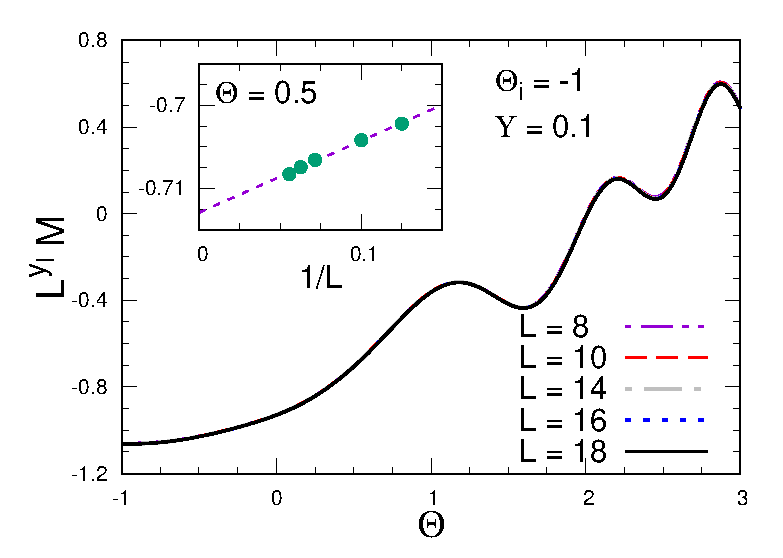
\includegraphics[width=0.65\columnwidth]{imm/IQY01ThX.eps}
  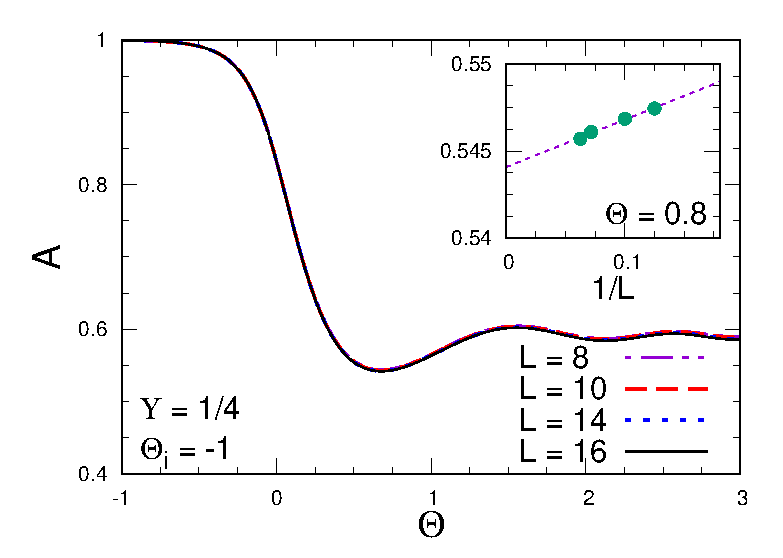
\includegraphics[width=0.65\columnwidth]{imm/IQY14ThA.eps}
  \caption{Dynamic FSS of the quantum Ising chain along the one-way KZ
    protocol at fixed $\Theta_i\equiv w_i L^{y_w}$.  We show results
    for the adiabaticity function $A(t,t_s,w_i,L)$ at fixed
    $\Upsilon=t_s/L^\zeta=1/4$ and $\Theta_i=-1$ up to $L=16$ (bottom)
    and the longitudinal magnetization $M(t,t_s,w_i,L)$ at fixed
    $\Upsilon=1/10$ and $\Theta_i=-1$ up to $L=18$ (top), versus
    $\Theta = t/t_s^\kappa$. The exponents $y_w$, $\zeta$, and
    $\kappa$ are reported in Eq.~(\ref{qisiexps}).  The approach to
    the large-$t_s$ asymptotic behavior is globally characterized by
    $O(1/L)$ corrections (apart from small superimposed wiggles), see
    for example the inset of the figures (where the line is drawn to
    guide the eyes).  }
  \label{dfssthetai}
\end{figure}


\begin{figure}[!htb]
\centering
  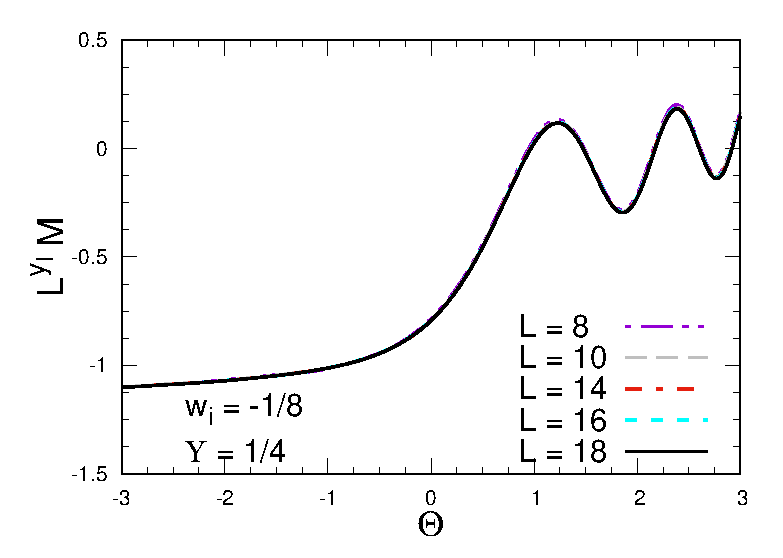
\includegraphics[width=0.65\columnwidth]{imm/IQY14W18X.eps}
  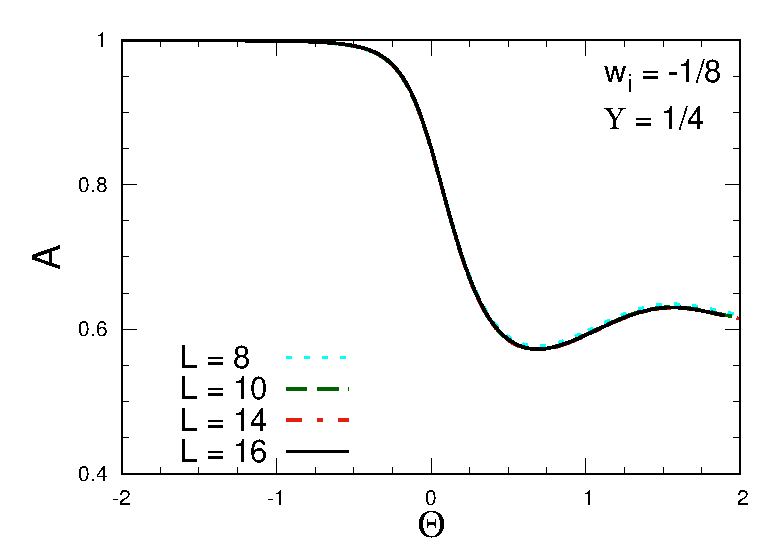
\includegraphics[width=0.65\columnwidth]{imm/IQY14W18A.eps}
  \caption{ Dynamic FSS of the quantum Ising chain along the one-way
    KZ protocol at fixed $w_i<0$.  We show the adiabaticity function
    $A(t,t_s,w_i,L)$ up to $L=16$ (bottom) and the longitudinal
    magnetization $M(t,t_s,w_i,L)$ up to $L=18$ (top), at fixed
    $\Upsilon=1/4$ and $w_i=-1/8$, versus $\Theta$. As explained in
    the text, the scaling behavior emerging at fixed $w_i<0$ matches
    that obtained in the $\Theta_i\to -\infty$ limit.}
  \label{dfsswi}
\end{figure}

The numerical analyses of quantum Ising chains (\ref{qisingmodel})
with a time-dependent longitudinal field is based on exact
diagonalization. The corresponding Schr\"odinger equation is solved
using a $4^{\rm th}$ order Runge-Kutta method. This approach allows us
to compute the out-of-equilibrium dynamics up to lattice size
$L\approx 16$, which, as we shall see, turns out to be sufficient to
achieve substantial evidence of the dynamic FSS outlined in the
previous sections.



We want to check the dynamic FSS put forward in Sec.~\ref{qfssoneway}.
In the case of the quantum 1D Ising model (\ref{isichoice}), the
exponents entering the definitions of the scaling variables
(\ref{KZscavar}) are 
\begin{equation}
y_w = 15/8\,,\qquad \zeta = 23/8\,,
\qquad \kappa = 8/23\,.
\label{qisiexps}
\end{equation}
Some results for the one-way protocol are reported in
Figs.~\ref{dfssthetai} and \ref{dfsswi}, respectively for the
adiabaticity function, defined in Eq.~(\ref{adtfunc}), and the
longitudinal magnetization, defined in Eq.~(\ref{magnt}), at fixed
$\Theta_i$ and $w_i$, for lattice sizes up to $L=16$ and $L=18$
respectively (this difference is due to the fact that the computation
of the adiabaticity function is heavier).  Although the system sizes
of the available results are only moderately large, we clearly observe
a collapse toward asymptotic scaling curves, thus a robust evidence of
the dynamic FSS outlined in Sec.~\ref{qfssoneway}.  In particular, the
dynamic FSS emerging from the data at fixed $w_i<0$ turns out to be
independent of the actual fixed value $w_i<0$, as predicted by the
scaling arguments reported in Sec.~\ref{qfssoneway} (in
Fig.~\ref{dfsswi} we only show results for $w_i=-1/8$, but we have
explicitly checked the independence of $w_i<0$ of the scaling
curves). We note that, as expected, the adiabaticity function
significantly drops crossing the quantum transition at finite values
of $\Upsilon$, while it remains close to one, i.e. the value
corresponding to adiabatic evolutions, for large values of $\Upsilon$.
We also  note that the data show that the convergence to the
asymptotic dynamic FSS is globally consistent with $O(1/L)$
corrections (apart from superimposed wiggles).


Analogous results are obtained for the quantum Kitaev wire, with
driving chemical potential.  The corresponding exponents,
cf. Eq.~(\ref{KZexps}), entering the definitions of the scaling
variables (\ref{KZscavar}), are
\begin{equation}
y_w = 1, \qquad \zeta = 2\,,\qquad \kappa =
1/2\,.
\label{kexps}
\end{equation}
The simpler {\em integrable} nature of the quantum Kitaev wire
(\ref{kitaev2}) allows us to easily consider much larger systems, up
to $L\approx 10^3$, using standard procedures after Fourier
transforming to the momentum space. Again the resulting data (not
shown) for the adiabaticity function, energy surplus, particle
density, and the two-point functions, cf. Eq.~(\ref{eq:corr}), nicely
support the dynamic FSS outlined in Sec.~\ref{qfssoneway}, see also
Ref.~\cite{RV-21}.



\subsection{Along the classical round-trip KZ protocol}
\label{clroundtrip}


\begin{figure}[!htb]
\centering
  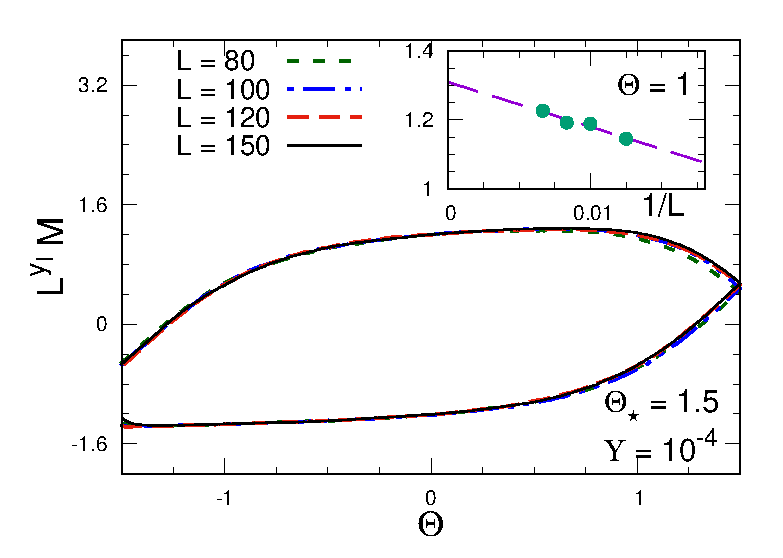
\includegraphics[width=0.65\columnwidth]{imm/isC2DT15Y104.eps}
  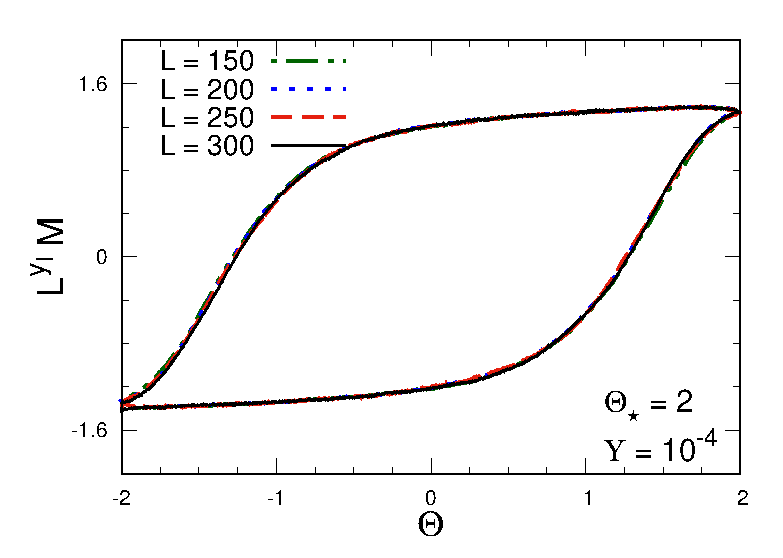
\includegraphics[width=0.65\columnwidth]{imm/isC2DT2Y104.eps}
  \caption{ Dynamic FSS behavior of $M(t,t_s,w_\star,L)$ for classical
    Ising model along the round-trip KZ protocol. Data are obtained at
    fixed $\Upsilon=10^{-4}$, and fixed $\Theta_\star = 1.5$ (top) and
    $\Theta_\star = 2$ (bottom), and are plotted versus $\Theta=w(t)
    t_s^{1-\kappa}$. The convergence is globally consistent with a
    $1/L$ behavior, see for example the inset of the top figure.  The
    values of the exponents $y_w$, $\zeta$, and $\kappa$ are reported
    in Eq.~(\ref{clisiexps}). Statistical errors are typically smaller
    than the thickness of the lines.}
  \label{roundtripM}
\end{figure}


\begin{figure}[!htb]
\centering
    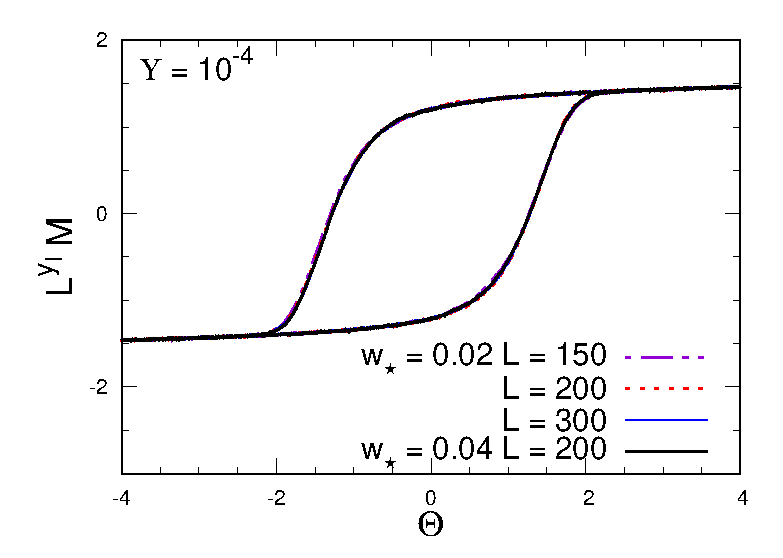
\includegraphics[width=0.65\columnwidth]{imm/isC2Dw002Y104.eps}
  \caption{ Dynamic FSS behavior of $M(t,t_s,w_\star,L)$ for the
    classical 2D Ising model along the round-trip KZ protocol for
    fixed $\Upsilon=10^{-4}$, and fixed $w_\star = 0.02$ and $w_\star
    = 0.04$. Statistical errors are typically smaller than the
    thickness of the lines. These results clearly support the
    predicted scaling behaviors, see Sec.~\ref{cfssKZroundtrip}, and
    their independence of the finite value of $w_\star>0$.  }
  \label{roundtripMW}
\end{figure}


\begin{figure}[!htb]
\centering
    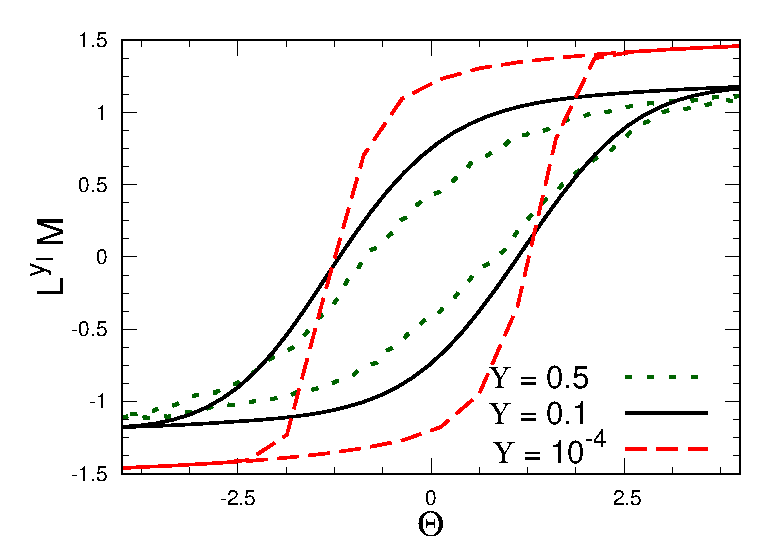
\includegraphics[width=0.65\columnwidth]{imm/isC2DL50.eps}
    \caption{Histeresis curves of the magnetization
      $M(t,t_s,w_\star,L)$ for the classical 2D Ising model along the
      round-trip KZ protocol for various values of fixed $\Upsilon$.
      They confirm that the hysteresis area decreases as $\Upsilon$
      increases. The curve for $\Upsilon=10^{-4}$ is taken from the
      data shown in Fig.~\ref{roundtripMW}, those for $\Upsilon=0.1$
      and $\Upsilon=0.5$ are obtained from simulations for $L=50$,
      whose size is already sufficient to provide a good approximation
      of the asymptotic large-$L$ scaling curves (note that Monte
      Carlo simulations becomes more demanding with increasing
      $\Upsilon$).}
  \label{roundtripMW2}
\end{figure}



The numerical analysis of the classical Ising model is based on
standard Monte Carlo simulations based on local Metropolis upgrading
procedures~\cite{Metropolis:1953am}, which provide a purely
relaxational dynamics without conserved quantities, that is model A
according to the standard classification reported in
Ref.~\cite{HH-77}.  The time unit of this dynamics is represented by a
global sweep of upgradings of all $L\times L$ spin variables. We
perform the single-site update sequentially, moving from one site to
one of its neighbours in a typewriter fashion.  The results along the
time-dependent protocols are obtained by averaging over a sample of
trajectories (tipically of order $10^3$), starting from an ensemble of
thermalized configurations at the initial parameter values. Also in
this case relatively large systems can be simulated, typically for
$L\gtrsim 10^2$.



The dynamic scaling arising from the one-way protocol is quite
analogous to that observed at quantum transitions, with corresponding
scaling behaviors, characterized by the static Ising critical exponents
supplemented by the purely relaxational dynamic exponent $z = 2.167(1)$.
The corresponding relevant exponents, cf. Eq.~(\ref{KZexps}), entering
the definitions of the scaling variables (\ref{KZscavar}), are
\begin{equation}
  y_w = 15/8\,,\quad \zeta = 4.0420(1)\,,\quad
  \kappa = 0.5361(1)\,.
  \label{clisiexps}
  \end{equation}
In the following we only report results for the round-trip KZ protocols,
taking also into account that its first part is equivalent to the
one-way KZ protocol.

The dynamic scaling behavior of the magnetization,
cf. Eq.~(\ref{genOscart}), is fully supported by the data reported in
Fig.~\ref{roundtripM}, for a fixed $\Upsilon=10^{-4}$ and two
different values of $\Theta_\star$.  Analogous results are obtained
for other values of $\Upsilon$.  As expected the round-trip cycle does
not close the curves for finite values of $\Upsilon$ and
$\Theta_\star$, see Eq.~(\ref{disacy}), leaving a finite gap between
the initial and final values of the cycle, i.e.
\begin{equation}
  {\cal M}^{(b)}(\Upsilon,-\Theta_{\star},\Theta_\star) -
  {\cal M}^{(a)}(\Upsilon,-\Theta_{\star},\Theta_\star)>0\,,
  \label{disacy2}
\end{equation}
which becomes smaller and smaller with increasing $\Theta_\star$.

As argued in Sec.~\ref{cfssKZroundtrip}, the outward and return
trajectories close in the large-$\Theta_\star$ limit, and therefore
for finite $w_\star>0$, giving rise to critical hysteresis phenomena.
This is clearly demonstrated by the results shown in
Fig.~\ref{roundtripMW} for two different finite values of $w_\star>0$,
whose scaling curves coincide. The outward and return curves for large
$|\Theta|$ tend to coincide, differing only within a finite interval
around $\Theta=0$, which becomes smaller and smaller with increasing
$\Upsilon$, and vanishes in the adiabatic limit
$\Upsilon\to\infty$. Such a dependence on $\Upsilon$ is demonstrated
by the curves reported in Fig.~\ref{roundtripMW2} showing the
magnetization hysteresis for various values of $\Upsilon$. They
confirm the scaling law (\ref{IAsca}) of the hysteresis area. Morever,
the data at small values of $\Upsilon$ hint at a convergence to a
constant for $\Upsilon\to 0$, which corresponds to the infinite-volume
limit.

As we shall see, these peculiar behaviors of round-trip protocols
developing scaling hysteresis do not have a quantum counterpart, being
strictly connected with the thermalizing relaxational dynamics of
classical models.


We also stress that the above hysteresis scenario arises from the
round-trip protocols between phases with short-ranged
correlations. More complicated situations are expected to occur when
round-trip protocols involve ordered phases, where coarsening
phenomena may drastically change the picture, in particular
along the return trip, in the large-$\Theta_\star$ limit.

\subsection{Along the quantum round-trip KZ protocol}
\label{qroundtrip}

\subsubsection{Scaling for finite $\Theta_\star$}
  \label{scafinthetastar}

\begin{figure}[!htb]
\centering
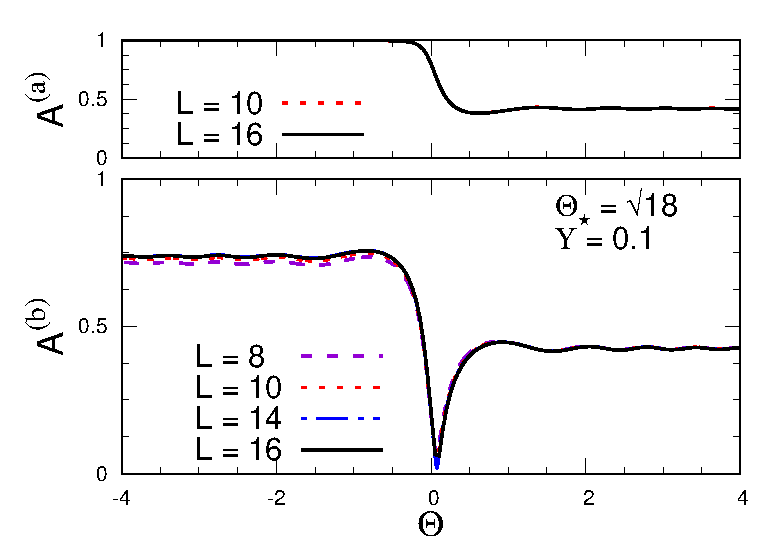
\includegraphics[width=0.65\columnwidth]{imm/headIQMY01ThA.eps}
\caption{ Round-trip dynamic FSS of the quantum Ising chain,
  cf. Eq.~(\ref{isichoice}, for a finite $\Theta_\star$.  We show
  results for the adiabaticity function $A(t,t_s,w_\star,L)$ at fixed
  $\Upsilon = t_s/L^\zeta= 0.1$ and $\Theta_\star = w_\star
  L^{1-\kappa}=3\sqrt{2}$, for the outward (top) and return (bottom)
  branches of the round-trip KZ protocol, versus
  $\Theta=w(t)L^{1-\kappa}$, for various size $L$ up to $L=16$.  The
  values of the exponents $y_w$, $\zeta$, and $\kappa$ are reported in
  Eq.~(\ref{qisiexps}).  The shown results clearly support the dynamic
  scaling behavior given in Eq.~(\ref{asca3}).  }
    \label{roundtripA}
\end{figure}


\begin{figure}[!htb]
\centering
  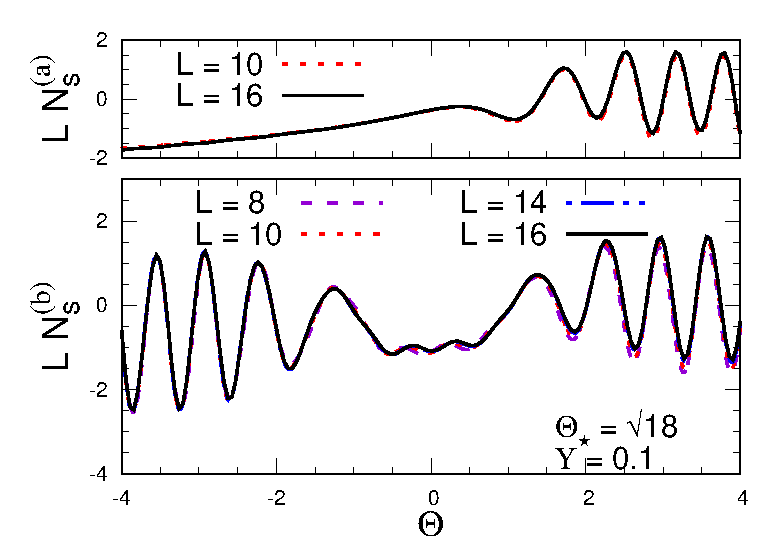
\includegraphics[width=0.65\columnwidth]{imm/headIQMY01ThZ.eps}
  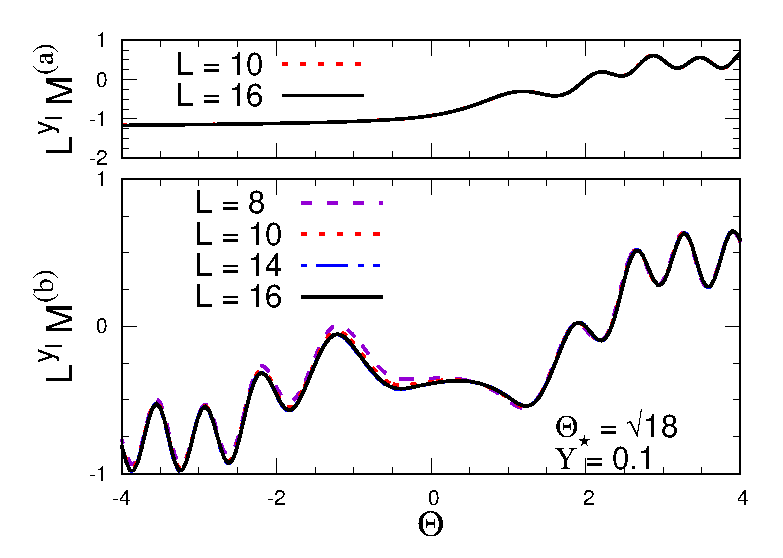
\includegraphics[width=0.65\columnwidth]{imm/headIQMY01ThX.eps}
  \caption{ Round-trip dynamic FSS of the longitudinal magnetization
    $M(t,t_s,w_\star,L)$ (bottom figure) and subtracted transverse
    magnetization $N_s(t,t_s,w_\star,L)$ (top figures),
    cf. Eq.~(\ref{subdef}), in the quantum Ising chain at fixed
    $\Upsilon=0.1$ and $\Theta_\star = 3\sqrt{2}$, for the outward
    (top) and return (bottom) branches of the round-trip KZ protocol,
    versus $\Theta$, for various size $L$ up to $L=16$.  The results
    clearly support the dynamic scaling behavior given in
    Eq.~(\ref{genOscart}).}
  \label{roundtripMN}
\end{figure}


\begin{figure}[!htb]
\centering
  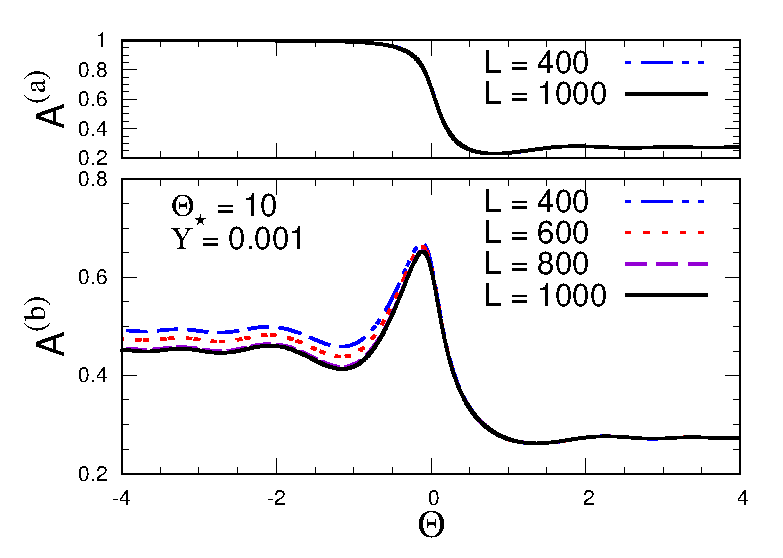
\includegraphics[width=0.65\columnwidth]{imm/headKITY0001Th10A.eps}
  \caption{ Round-trip dynamic FSS within the quantum Kitaev wire for
    a finite $\Theta_\star$.  We show results for the adiabaticity
    function $A(t,t_s,w_\star,L)$ at fixed $\Upsilon =t_s/L^\zeta =
    0.001$ and $\Theta_\star = w_\star L^{1-\kappa}=10$, for the
    outward (top) and return (bottom) branches of the round-trip KZ
    protocol, versus $\Theta=w(t)L^{1-\kappa}$, for various size $L$
    up to $L=1000$.  The values of the exponents $y_w$, $\zeta$, and
    $\kappa$ are reported in Eq.~(\ref{kexps}).  The numerical results
    clearly support the dynamic scaling behavior given in
    Eq.~(\ref{asca3}).}
  \label{roundtripdfssA}
\end{figure}

\begin{figure}[!htb]
\centering
  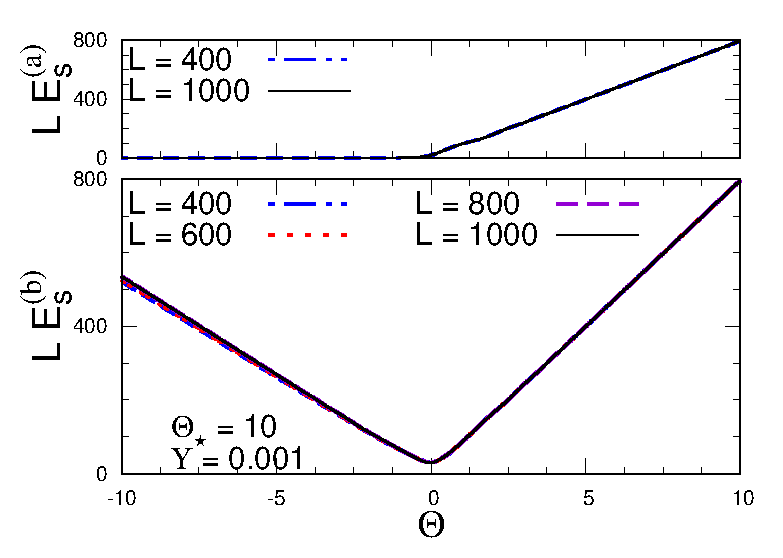
\includegraphics[width=0.65\columnwidth]{imm/headKITY0001Th10E.eps}
  \caption{ Round-trip dynamic FSS within the quantum Kitaev wire for
    a finite $\Theta_\star$.  We show results for the surplus energy
    $E_s(t,t_s,w_\star,L)$ defined in Eq.~(\ref{etdiff}), at $\Upsilon
    =t_s/L^\zeta = 0.001$, and $\Theta_\star = w_\star
    L^{1-\kappa}=10$, for the outward (top) and return (bottom)
    branches of the round-trip KZ protocol, versus
    $\Theta=w(t)L^{1-\kappa}$, for various size $L$ up to $L=1000$.
    The results clearly support
  the dynamic scaling behavior given in Eq.~(\ref{esca3}).
    }
  \label{roundtripdfssE}
\end{figure}


\begin{figure}[!htb]
\centering
  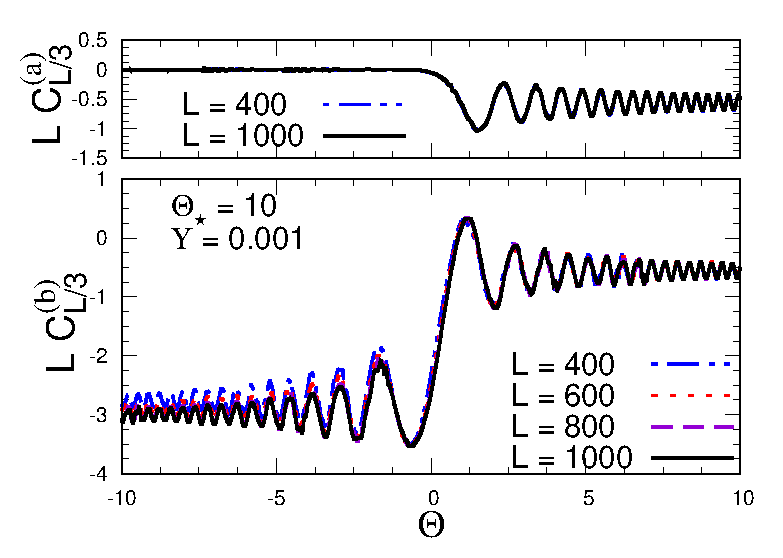
\includegraphics[width=0.65\columnwidth]{imm/headKITY0001Th10C.eps}
  \caption{ Round-trip dynamic FSS within the quantum Kitaev wire for
    a finite $\Theta_\star$.  We show results for the two-point
    function $C(x,t,t_s,w_\star,L)$, cf. Eq.~(\ref{eq:corr}), at fixed
  $X=x/L=1/3$, $\Upsilon =t_s/L^\zeta = 0.001$, and $\Theta_\star =
  w_\star L^{1-\kappa}=10$, for the outward (top) and return (bottom)
  branches of the round-trip KZ protocol, versus
  $\Theta=w(t)L^{1-\kappa}$, for various size $L$ up to $L=1000$.
  }
  \label{roundtripdfssC}
\end{figure}




To begin with, we show results for round-trip KZ protocols for the
quantum Ising chain, cf. Eq.~(\ref{isichoice}), when keeping
$\Theta_\star$ finite, see Figs.~\ref{roundtripA}
and \ref{roundtripMN}, respectively for the adiabaticity function, the
longitudinal and transverse magnetizations.  Analogous results are
obtained for other values of $\Upsilon$ and $\Theta_\star$. They
nicely support the scaling behaviors put forward in
Sec.~\ref{qfssKZroundtrip}.  Analogous results are obtained for the
quantum Kitaev wire, cf. Eq.~(\ref{kitchoice}), see for example the
results shown in Figs.~\ref{roundtripdfssA}, \ref{roundtripdfssE}, and
\ref{roundtripdfssC}, respectively for the adiabaticity function, the
surplus energy $E_s$ defined in Eq.~(\ref{etdiff}), and the two point
function defined in Eq.~(\ref{eq:corr}). They nicely support the
dynamic FSS at fixed finite $\Theta_\star$.



\subsubsection{The limit $\Theta_\star\to\infty$}
  \label{scafinthetastarinf}

\begin{figure}[!htb]
\centering
  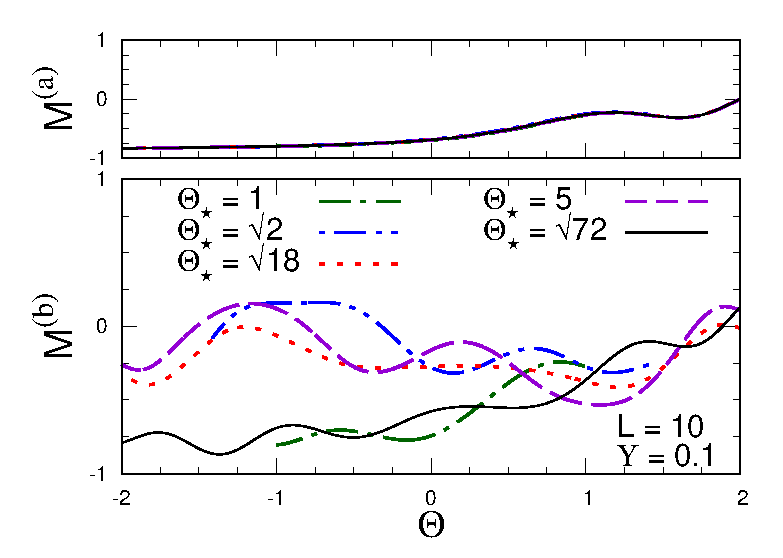
\includegraphics[width=0.65\columnwidth]{imm/headDiffThsY01L10X.eps}
 \caption{ Behavior of $M(t,t_s,w_\star,L)$ for fixed $L = 10$,
   $\Upsilon = 0.1$ for the one way trip (top figure) and for the
   return trip (bottom figure), versus $\Theta$, for various
   $\Theta_\star$ up to $\Theta_\star = 6\sqrt{2}$.  We note that
   along the outward path the convergence is large-$\Theta_\star$
   convergence is rapid (it is essentially related to the convergence
   with respect to $\Theta_i=-\Theta_\star$ of the one-way protocol),
   along the return path the curves do not appear to approach a
   large-$\Theta_\star$ limit.}
  \label{diffThetaStar}
\end{figure}


We now discuss the large-$\Theta_\star$ limit, or equivalently the
case in which we keep $w_\star>0$ fixed in the round-trip protocols.
This limit turns out to be quite problematic in quantum round-trip KZ
protocols.

  
Some hints at the absence of a well defined large-$\Theta_\star$ limit
of the dynamic scaling behavior are shown by the plots of
Fig.~\ref{diffThetaStar} reporting the longitudinal magnetization of a
quantum Ising system of size $L=10$ for various $\Theta_\star$, whose
return paths do not show any apparent convergence when increasing
$\Theta_\star$.



\begin{figure}[!htb]
\centering
  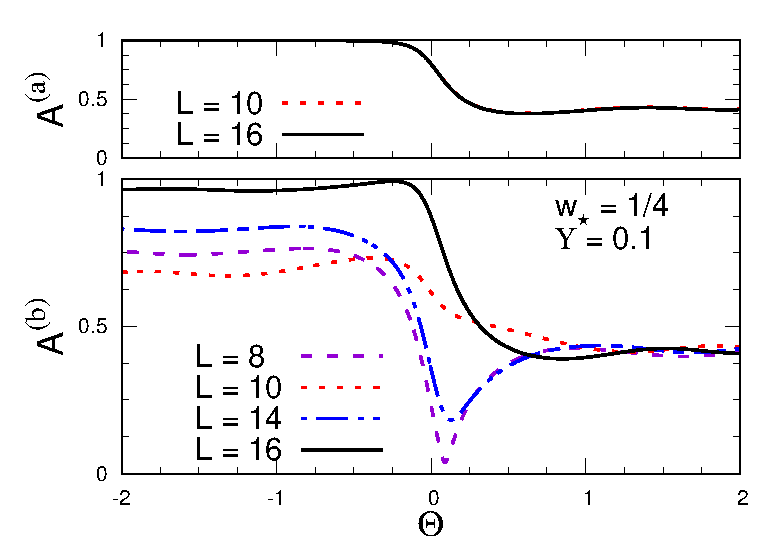
\includegraphics[width=0.65\columnwidth]{imm/headIQMY01W025A.eps}
  \caption{ The adiabaticity function $A(t,t_s,w_\star,L)$ of quantum
    Ising chains along round-trip protocols, for fixed $\Upsilon =
    0.1$ and $w_\star = 1/4$, for the outward (top) and return
    (bottom) branches of the round-trip protocol, versus $\Theta$, for
    various size $L$ up to $L=16$.  }
  \label{roundtripAW}
\end{figure}


\begin{figure}[!htb]
\centering
  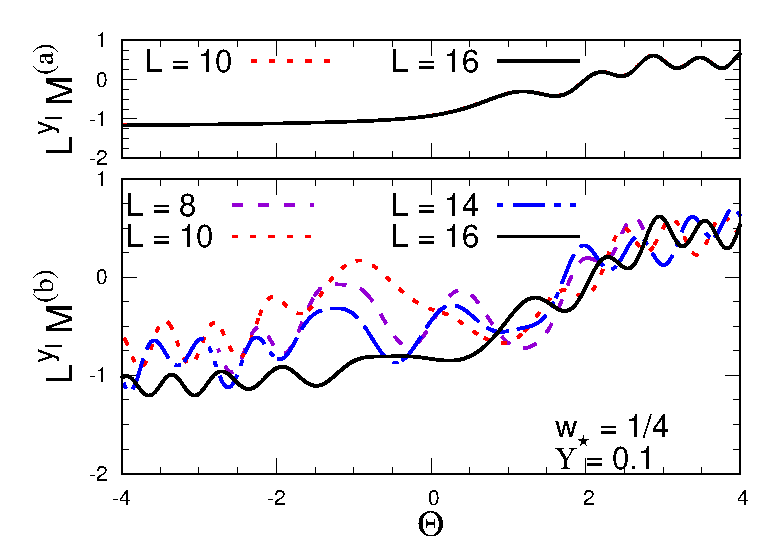
\includegraphics[width=0.65\columnwidth]{imm/headIQMY01W025X.eps}
 \caption{ The longitudinal magnetization $M(t,t_s,w_\star,L)$ along
   the round-trip protocol, for fixed $w_\star = 1/4$, $\Upsilon =
   0.1$ for the outward (top) and return (bottom) branches of the
   round-trip protocol, versus $\Theta$, for various size $L$ up to
   $L=16$.  }
  \label{roundtripMxW}
\end{figure}


%\begin{figure}[!htb]
%\centering
%  \includegraphics[width=0.65\columnwidth]{imm/headIQMY01W025Z.eps}
% \caption{ The subtracted transverse magnetization
%   $N_s(t,t_s,w_\star,L)$ along the round-trip protocol, for fixed
%   $w_\star = 1/4$, $\Upsilon = 0.1$ for the outward (top) and return
%   (bottom) branches of the round-trip protocol, versus $\Theta$, for
%   various size $L$ up to $L=16$.  }
%  \label{roundtripMzW}
%\end{figure}





\begin{figure}[!htb]
\centering
  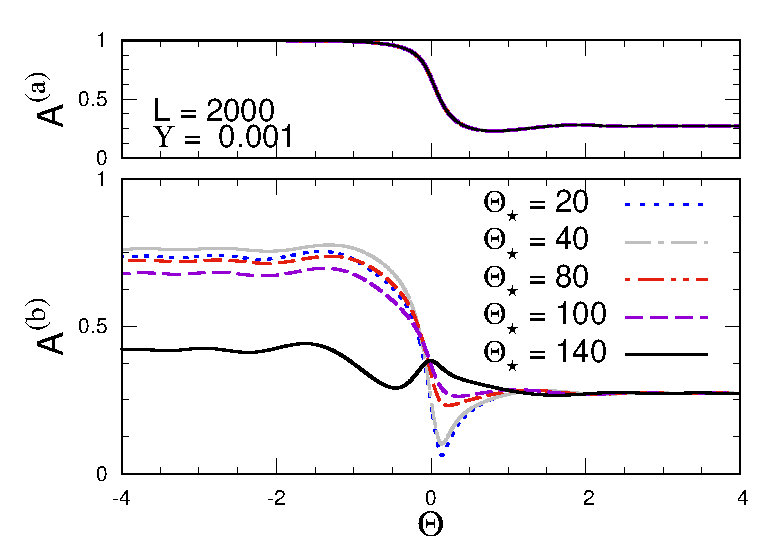
\includegraphics[width=0.65\columnwidth]{imm/headKITY0001L2000A.eps}
 \caption{The adiabaticity function $A(t,t_s,w_\star,L)$ for the
   quantum Kitaev wire at $L=2000$ and $\Upsilon = 0.001$ for the
   outward (top) and return (bottom) branches of the round-trip KZ
   protocol, versus $\Theta$, for various $\Theta_\star$ up to
   $\Theta_\star = 140$.  We note that along the outward path the
   convergence is large-$\Theta_\star$ convergence is rapid (it is
   essentially related to the convergence with respect to
   $\Theta_i=-\Theta_\star$ in the one-way KZ protocol), along the
   return path the curves do not appear to approach a
   large-$\Theta_\star$ limit.}
  \label{diffThetaStarA}
\end{figure}

The return trajectories keeping $w_\star>0$ fixed do not show evidence
of convergence in the large-$L$ dynamic scaling limit.  This is shown
by the curves of the adiabaticity function along the return branch of
the round-trip protocol, see Fig.\ref{roundtripAW}, for $w_\star=1/4$
and $\Upsilon=0.1$.  While convergence is clearly observed along the
outward part, as expected because the one-way protocol showed a well
defined limit in the large-$|\Theta_i|$ limit, the return pattern does
not show a stable convergence pattern. The same behavior is also shown
by the longitudinal and transverse magnetizations $M$ and $N$, see for
example Fig.~\ref{roundtripMxW}.  Analogous results are also obtained
for the quantum Kitaev wire, see Fig.~\ref{diffThetaStarA}, where we
report results for the adiabaticity function at $\Upsilon=0.001$ and
various large values of $\Theta_\star$, for a large lattice size
$L=2000$.

Actually, such an instability appears quite similar to that emerging
in analogous round-trip protocols within two-level systems.  They are
discussed in App.~\ref{LZlike}. Similarly to the 
Landau-Zener problem~\cite{LZeff}, we consider a time-dependent two-level
Hamiltonian
\begin{equation}
  H_{2\ell}(t) = - \beta(t) \sigma^{(3)}
  + {\Delta\over 2} \sigma^{(1)}\,,
\label{hrdef2}
\end{equation}
where $\Delta$ is a constant, 
\begin{eqnarray}
  \beta(t) = {{\cal T}(t)\over t_s}\quad
       {\rm for}\;\; t_i=-t_\star \le t \le 3t_\star\,,
\label{betadef}
\end{eqnarray}
and $ {\cal T}(t) = t_\star - |t-t_\star|$ is the triangular
function. The quantities $\tau={\cal T}(t)/\sqrt{t_s}$ and
$\tau_\star=t_\star/\sqrt{t_s}$ play the same role of the scaling
variables $\Theta$ and $\Theta_\star$ describing the round-trip KZ
protocols in quantum many-body systems. The corresponding
Schr\"odinger functions can be analytically solved in terms 
of parabolic cylinder functions $D_\nu(x)$~\cite{VG-96}, see
App.~\ref{LZlike}.

The resulting behavior of the expectation values of $\sigma^{(3)}$ and
the adiabatic function show that the large-$\tau_\star$ limit is
problematic, being characterized by large $O(1)$ oscillations with
frequencies increasing proportionally to $\tau_\star$, roughly. See
App.~\ref{LZlike} for details.  They turn out to be related to the
rapid changes of the relative phase between the relevant states of the
two-level system at the extremal values $\tau=\tau_\star$ when
$\tau_\star$ becomes large, increasing as $\tau_\star^2$. Since the
quantum evolution along the return trajectory turns out to be very
dependent on such phase, it becomes extremely sensitive to the value
of $\tau_\star$, showing analogous oscillations. As a consequence, the
value of all observables along the return trajectory, from
$\tau=\tau_\star$ down to the return point $\tau = - \tau_\star$, do
not show a well defined limit for $\tau_\star\to\infty$.  The size of
the oscillations depend on the value of the scaling variable
$\Upsilon$, and tend to be suppressed in the adiabatic limit
$\Upsilon\to\infty$.

\begin{figure}[!htb]
\centering
  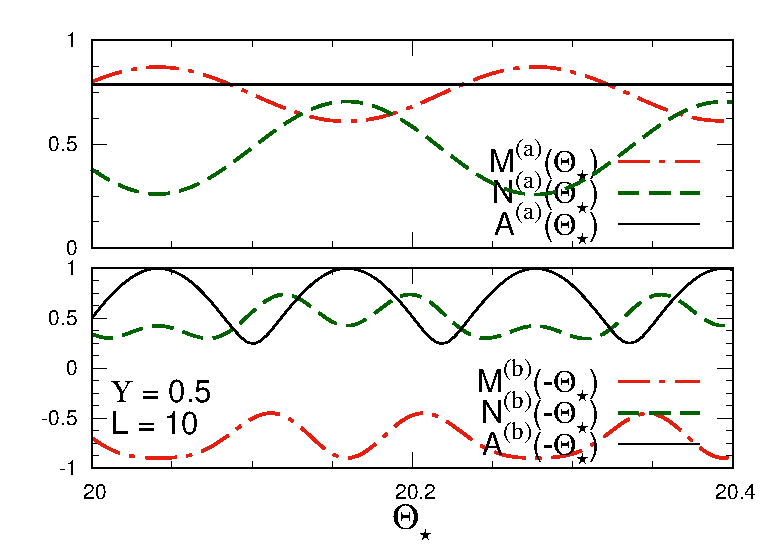
\includegraphics[width=0.45\columnwidth]{imm/diffThstaru50s20l10.eps}
  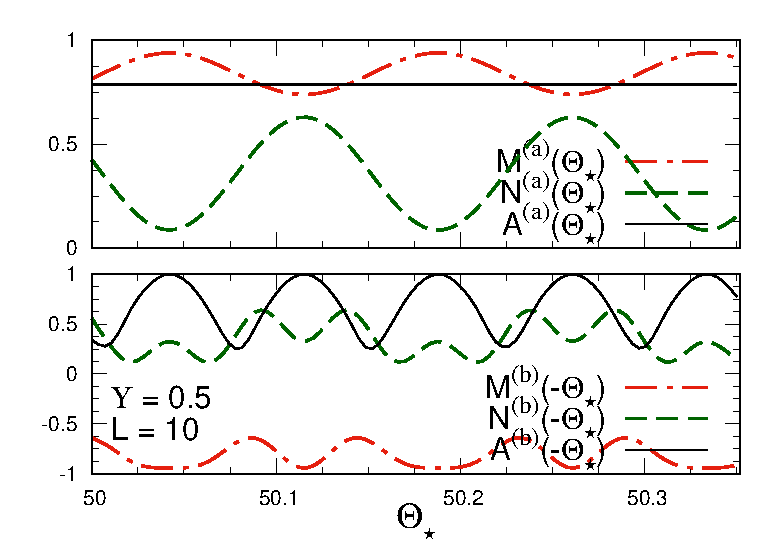
\includegraphics[width=0.45\columnwidth]{imm/diffThstaru50s50l10.eps}
 \caption{ Results for $M,\, N$ and $A$ for fixed $L = 10$, $\Upsilon
   = 0.5$ versus $\Theta_\star$, close to $\Theta_\star = 20$ (top
   figure) and $\Theta_\star = 50$ (bottom figure). In each figure,
   the top plot the values of $M^{(a)}$, $N^{(a)}$ and $A^{(a)}$ at
   the end of the outward branch, corresponding to
   $\Theta=\Theta_\star$, while the bottom plot shows the values of
   $M^{(b)}$, $N^{(b)}$ and $A^{(b)}$ at the end of the return branch,
   corresponding to $\Theta=-\Theta_\star$. The comparison of the top
   and bottom figures show that the oscillations tend to become more
   frequent with increasing $\Theta_\star$ (note that the interval of
   the abscissa is different).  Analogous results are obtained for
   other values of $\Upsilon$.}
  \label{roundtripDiffTheta}
\end{figure}

%\begin{figure}[!htb]
%  \centering
%  \includegraphics[width=0.65\columnwidth]{imm/diffThstaru10s25l10.eps}
%  \includegraphics[width=0.65\columnwidth]{imm/diffThstaru10s50l10.eps}
% \caption{ Results for $M,\, N_s$ and $A$ for fixed $L = 10$,
%   $\Upsilon = 0.1$ versus $\Theta_\star$, close to $\Theta_\star =
%   20$ (top figure) and $\Theta_\star = 50$ (bottom figure). In each figure,
%   the top plot shows the one way trip, while the bottom plot shows
%   the return trip.   }
%  \label{roundtripDiffTheta2}
%\end{figure}



\begin{figure}[!htb]
\centering
%  \includegraphics[width=0.65\columnwidth]{imm/diffThstaru0001T35l40.eps}
   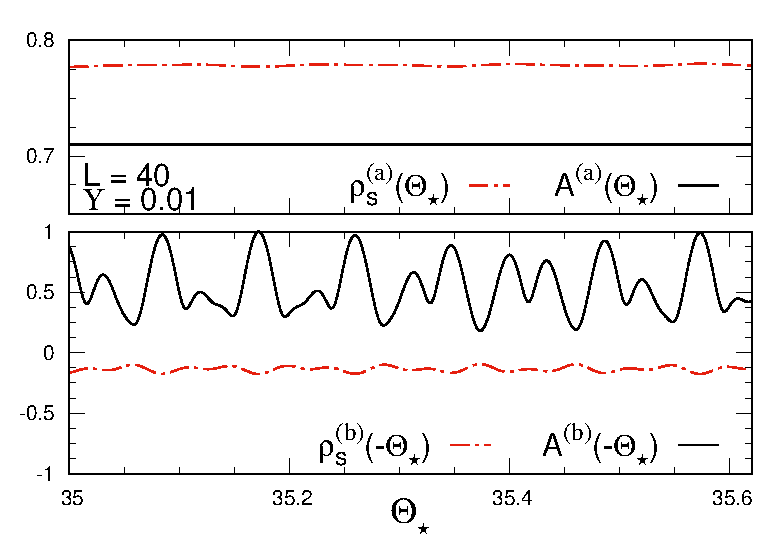
\includegraphics[width=0.45\columnwidth]{imm/diffThstaru001T35l40.eps}
  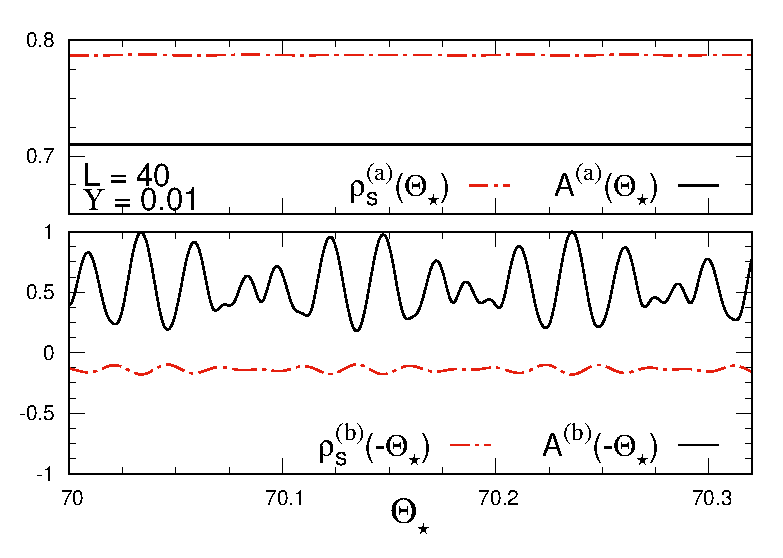
\includegraphics[width=0.45\columnwidth]{imm/diffThstaru001T70l40.eps}
  \caption{ Behavior of the subtracted particle density $\rho_s$,
    cf. Eq.~(\ref{rhot}), and the adiabaticity function $A$ for the
    Kitaev wire, for fixed $L = 40$, $\Upsilon = 0.01$ versus
    $\Theta_\star$, close to $\Theta_\star = 70$ (bottom figure) and
    $\Theta_\star=35$ (top figure).  In each figure, the top plot the
    values of $\rho_s^{(a)}$ and $A^{(a)}$ at the end of the outward
    branch, corresponding to $\Theta=\Theta_\star$, while the bottom
    plot shows the values of $\rho_s^{(b)}$ and $A^{(b)}$ at the end
    of the return branch, corresponding to $\Theta=-\Theta_\star$.
    Again, the comparison of the top and bottom figures show that the
    oscillations tend to become more frequent with increasing
    $\Theta_\star$.  }
  \label{roundtripDiffThetaAR}
\end{figure}



We observe a similar behavior in the quantum many-body systems.  This
scenario is demonstrated by the results shown in
Fig.~\ref{roundtripDiffTheta}, where we report the values of $A$, $M$,
and $N_s$ at end of the outward branch and at the end of the return
branch for some interval of values of $\Theta_\star$, around large
values of $\Theta_\star$ and fixed $L=10$.  Similarly to the results
obtained for two-level model, the observables at the end of the
outward branch oscillate, with a frequency that becomes larger and
larger with increasing $\Theta_\star$, and the oscillations observed
after the whole cycle are strongly correlated to those at the end of
the first branch, doubling the frequency.  Analogous results are
obtained for other values of $\Upsilon$.  We also note that the
oscillations tend to be suppressed in the adiabatic
$\Upsilon\to\infty$ limit. We believe that this extreme sensitivity to
$\Theta_\star$ makes also problematic the large-$L$ limit after the
limit $\Theta_\star\to\infty$ shown by the numerical data.

Similar results are also obtained for the quantum Kitaev wire, see
Fig.~\ref{roundtripDiffThetaAR} where we show results for the
adiabaticity function and the particle density.  In this case the
values at the end of the outward way appear quite stable, but the
return way is characterized again by large (less regular) oscillations
with larger and larger frequencies with increasing $\Theta_\star$.


On the basis of the above results, we conclude that in quantum
many-body systems the large-$\Theta_\star$ limit of the dynamic KZ
scaling does not apparently exist along the return trajectories,
showing similarities with the behavior of two-level model
(\ref{hrdef2}) subject to round-trip protocols. We believe that this
issue deserves further investigation, for example addressing the
possibility of obtaining well defined scaling behavior after some
average procedures over the oscillations induced by large valyes of
$\Theta_\star$, to obtained a well defined large-$\Theta_\star$ limit.

However, we stress that the dynamic scaling behavior is nicely
observed when keeping $\Theta_\star$ fixed, even along the return
trajectory. This is related to fact that, when keeping $\Theta_\star$
fixed, the time scaling variable $\Theta$ remains finite, therefore
the time variable is always rescaled consistently with the time scale
of the equilibrium quantum transition, provided by the inverse gap at
the transition $\Delta \sim L^{-z} \sim \lambda^{-z}$. As a
consequence, the the variation of $w(t)$ gets limited within a small
interval $\delta_w$ around the transition, which becomes smaller and
smaller in the large-size limit, as $\delta_w \sim L^{-y_w}$.
